\documentclass[a4paper,twoside,12pt,hidelinks]{article}
\usepackage{float}
\usepackage{listings}
\usepackage[titletoc]{appendix}
\usepackage[justification=centering]{caption}
\setlength{\belowcaptionskip}{-5pt}
\usepackage{subcaption}
\lstset{aboveskip=5pt,belowskip=8pt}
\usepackage[a4paper,left=1.25in,right=1.25in,top=1in,bottom=1in]{geometry}
\usepackage[parfill]{parskip}
\usepackage{graphicx}
\usepackage[export]{adjustbox}
\usepackage{siunitx}
\usepackage{amsmath,amssymb}
\usepackage{mathtools}
\usepackage{commath}
\usepackage{multirow}
\usepackage{setspace}
\usepackage{tabularx}
\newcolumntype{Y}{>{\centering\arraybackslash}X}
\usepackage{pdflscape}
\usepackage[nodayofweek,level]{datetime}
\usepackage{wrapfig}
\graphicspath{{figures/}}
\usepackage[raggedright]{titlesec}
\setcounter{secnumdepth}{4}
\titleformat{\paragraph}
{\normalfont\normalsize\bfseries}{\theparagraph}{1em}{}
\titlespacing*{\paragraph}
{0pt}{3.25ex plus 1ex minus .2ex}{1.5ex plus .2ex}
\usepackage[nottoc]{tocbibind}
\usepackage[numbered]{matlab-prettifier}
\usepackage{IEEEtrantools}
\definecolor{lstgrey}{rgb}{0.97,0.97,0.97}
\lstdefinestyle{mymatstyle}{%
  style=Matlab-editor,
  basicstyle=\scriptsize,
  numbers=left,
  numberstyle=\scriptsize,
  literate={\ \ }{{\ }}1,
  backgroundcolor=\color{lstgrey},
  frame=single,
  xleftmargin=0.5cm,
  xrightmargin=0.25cm,
  numbersep=7pt
}
\usepackage{notoccite}
\usepackage[colorlinks=false]{hyperref}
\usepackage{cleveref}
\crefname{paragraph}{section}{sections}
\Crefname{paragraph}{Section}{Sections}


\usepackage{fancyhdr}
\usepackage[intoc]{nomencl}
\makenomenclature

\titlespacing\section{0pt}{6pt plus 4pt minus 2pt}{0pt plus 2pt minus 2pt}
\titlespacing\subsection{0pt}{6pt plus 4pt minus 2pt}{0pt plus 2pt minus 2pt}
\titlespacing\subsubsection{0pt}{6pt plus 4pt minus 2pt}{0pt plus 2pt minus 2pt}
\titlespacing\paragraph{0pt}{6pt plus 4pt minus 2pt}{0pt plus 2pt minus 2pt}

\begin{document}
\bstctlcite{IEEEexample:BSTcontrol}
\nomenclature{DOA}{Direction of Arrival}
\nomenclature{TF}{Time-frequency}
\nomenclature{BSS}{Blind Source Separation}
\nomenclature{TDOA}{Time Difference of Arrival}
\nomenclature{RT$_{60}$}{Reverberation Time}
\nomenclature{DRR}{Direct-to-Reverberant Ratio} 
\nomenclature{GSC}{Generalised Sidelobe Canceller}
\nomenclature{FCM}{Fuzzy $c$-means Clustering}
\nomenclature{MUSHRA}{MUltiple Stimuli with Hidden Reference and Anchor} 
\nomenclature{SDR}{Signal-to-Distortion Ratio}
\nomenclature{SNR}{Signal-to-Noise Ratio}
\nomenclature{SIR}{Source-to-Interference Ratio}
\nomenclature{SAR}{Sources-to-Artifacts Ratio}
\nomenclature{PESQ}{Perceptual Evaluation of Speech Quality} 
\nomenclature{STOI}{Short-time Objective Intelligibility}
\nomenclature{RIR}{Room Impulse Response}
\nomenclature{LTI}{Linear Time-invariant}
\nomenclature{DSB}{Delay-Sum Beamformer}
\nomenclature{STFT}{Short-time Fourier Transform}
\nomenclature{wFCM}{Weighted Fuzzy $c$-means Clustering}
\nomenclature{wCFCM}{Weighted Contextual Fuzzy $c$-means Clustering}
\nomenclature{MVDR}{Minimum Variance Distortionless Response}
\nomenclature{MOS-LQO}{Mean Opinion Score - Listening Quality Objective}
\nomenclature{DNN}{Deep Neural Network}
\begin{titlepage}
                % \newgeometry{top=25mm,bottom=25mm,left=38mm,right=32mm}
                \setlength{\parindent}{0pt}
                \setlength{\parskip}{0pt}
                % \fontfamily{phv}\selectfont

                {
                                \Large
                                \raggedright
                                Imperial College London\\[17pt]
                                Department of Electrical and Electronic Engineering\\[17pt]
                                Final Year Project Report 2018\\[17pt]
 
                }

                \rule{\columnwidth}{3pt}
                \vfill
                \centering
                  \includegraphics[width=0.7\columnwidth,height=60mm,keepaspectratio]{communications}
                \vfill
                \setlength{\tabcolsep}{0pt}

                \begin{tabular}{p{40mm}p{\dimexpr\columnwidth-40mm}}
                                Project Title: & \textbf{Audio Signal Zoom for Small Microphone Arrays} \\[12pt]
                                Student: & \textbf{Chi Hang Leung} \\[12pt]
                                CID: & \textbf{00978321} \\[12pt]
                                Course: & \textbf{4T} \\[12pt]
                                Project Supervisor: & \textbf{Dr Patrick Naylor} \\[12pt]
                                Second Marker: & \textbf{Mr Mike Brookes} \\
                \end{tabular}
\end{titlepage}
\pagebreak
\clearpage
\thispagestyle{empty}
\null
\clearpage
\pagenumbering{roman}
\setcounter{page}{1}
\vspace*{2in}
\spacing{1.15}
\renewcommand{\abstractname}{\Large Abstract}
\begin{abstract}
\noindent\normalsize
Nowadays, often do people use their smartphones or cameras to capture videos of the memorable moments. It is convenient to visually zoom in towards the subject of interest and suppress the unwanted interferences. A problem is then posed - whether the same could be achieved in audio terms. Despite demonstrating a high spatial selectivity, current approaches usually require large microphone arrays. This motivates the project to explore and develop alternative approaches that are suitable for small devices like smartphones. 
\\\\
This report firstly outlines the process of software simulation to capture audio containing two persons talking. Using the synthetic audio data, the report proposes several audio zooming algorithms, including time-frequency masking, beamforming and machine learning. The performance of the zooming algorithms under different reverberant conditions is then evaluated in terms of speech quality and intelligibility through both subjective and objective metrics. The report ultimately provides an insight on the practicality of implementing the algorithms on smartphones.

\end{abstract}
\newpage
\vspace*{2in}
\renewcommand{\abstractname}{\Large Acknowledgements}
\begin{abstract}
\noindent\normalsize
I would like to firstly express my gratitude towards my project supervisor, Dr. Patrick Naylor, for his insightful advice and guidance throughout the project.
\\\\
I would also like to thank the Speech and Audio Processing Laboratory for providing me with the anechoic audio data needed in the project, and Mr. Aidan Hogg for his help with the evaluation section of the project. 
\\\\
Lastly, I would like to thank my parents for their unconditional support through the years. I also wish to express my great appreciation to Mr. Chak Man Tang on helping with the visualisation of the project concept, as well as whom took part in the listening test. 
\end{abstract}
\newpage
\setcounter{tocdepth}{3}
\spacing{0.75}
\tableofcontents
\newpage
\singlespacing
\listoffigures
\listoftables
\newpage
\onehalfspacing
\renewcommand{\nomname}{List of Abbreviations}
\printnomenclature[1in]
\newpage
\spacing{1.15}
\pagenumbering{arabic}
\setcounter{page}{1}
\pagestyle{fancy}
\fancyhf{}
\let\Subsectionmark\subsectionmark
\def\subsectionmark#1{\def\Subsectionname{#1}\Subsectionmark{#1}}
\rhead{\thepage}
\cfoot{}
\lhead{\itshape\nouppercase{\thesubsection~~\Subsectionname}}
\setlength{\headheight}{1cm}
\setlength{\headsep}{14pt}
\section{Introduction}
Often one would take videos using their smartphones to capture the precious moments, such as parties and ceremonies. However, inevitably there would be interference, where one would zoom the camera towards the point of interest to avoid the unwanted subjects. A similar question aroused - whether one can make the sound of the speaker of interest closer in the context of smartphones. 

This problem resonates with the well-known `Cocktail Party Problem' illustrated by Colin Cherry in 1953 \cite{Cherry1953SomeEars}. Human brains have the ability to amplify the sound coming from a certain direction using their phase difference of arrival to two ears. Hence, under noisy environments such as cocktail party, with a lot of people speaking, the person one is chatting with is still audible. Over the years, different signal processing techniques have been developed to try replicating the processing by human ears and brains to microphones and computer. \cite{Mitchell1971SignalEffect} Despite being an established technique to achieve audio zoom, classical beamforming technique requires large microphone arrays typically to provide a narrow and precise beam. For small devices like phones in this project's context, developing alternative approaches is required.

Hence, this project seeks to investigate both classical and novel or a combination of algorithms to achieve acoustic zooming in the context of smartphones. The purpose of the project is to capture audio samples containing multiple speakers, which then could be used to develop an algorithm that can zoom (in audio terms) towards one selected sound source. The nature of the project is software-based, with MATLAB being the main platform for development. The code and results of the project is available on \url{https://github.com/chl214/FYP}\footnote{Anechoic speech data used in the project is excluded from the repository due to confidentiality concern}
\begin{figure}[H]
\centering
\includegraphics[width=0.49\textwidth]{audiozoom}
\caption{Concept of Audio Zoom on Smartphones}
\end{figure}

\subsection{Scope and Aims}
The stated problem can be decomposed into two parts, one part as identifying the direction of the speaker with respect to the smartphone, with the next part being processing the received signals to zoom into a speaker of interest and suppress the other. In the context of this project, the focus is to develop the algorithm for the latter part. Hence, it is assumed throughout the project that the direction of arrival (DOA) of the speech from the speakers to the microphones, as illustrated in \Cref{fig:doa}, are known.

The aims of the project include the following: 
\begin{itemize}
\item Capturing audio samples containing more than one person talking in real life with different reverberant conditions, and potentially with background noises
\item Developing and Experimenting algorithms that can zoom (in audio terms) towards the speaker of interest
\item Evaluating and comparing the performances of the algorithms (e.g. in terms of speech quality and intelligibility)
\end{itemize}

An important point to note here is regarding to the first aim to capture audio examples. Instead of real-life recording using smartphones, a room acoustics simulation environment using anechoic speeches as input is preferred. This would allow a more rapid verification environment for the algorithm, as one can easily modify parameters such as speakers and receivers position, degree of reverberation and size of the room, and generate a new set of test data. While real-life data would be the ultimate goal of the project, the flexibility and rapidness in prototyping leads to the selection of software simulation.

Also, in this project, processing are assumed to be done offline, i.e. after the audio capturing has been completed. This assumption allows the processing technique to not be in real-time, hence more freedom in developing the algorithm, where it can look into the `future' data, not only the past.

Despite the ultimate aim to apply the acoustic zoom in scenarios containing multiple speakers, the scope of the project would be focusing on the cases involving two speakers, with the vision that the algorithm can be potentially extended to a multi-source environment. Besides, as the initiative of the project is to apply the acoustic zoom algorithm on mobile phones, the microphones set-up should comply the physical constraint of mobile phones. Typically, mobile phones have a dual-omnidirectional-microphone set-up \cite{Jeub2012NoiseDifferences}, with its dimension being around 15cm x 8cm, as seen from \Cref{fig:mobilephone}. Hence, the number of omnidirectional microphones is chosen to be two, and the separation has to be confined within the mentioned dimensions. 

\begin{figure}[H]
\centering
\begin{subfigure}[t]{0.49\textwidth}
\includegraphics[width=0.9\textwidth]{mobilephone}
\caption{Example of microphones location in a smartphone. (From \cite{Jeub2012NoiseDifferences})}
\label{fig:mobilephone}
\end{subfigure}
\begin{subfigure}[t]{0.49\textwidth}
\includegraphics[width=0.9\textwidth]{doa}
\caption{Illustration of direction of arrival of a sound wave}
\label{fig:doa}
\end{subfigure}
\caption{Illustration of the set up adopted in the project}
\end{figure}

\subsection{Project Breakdown and Requirements Capture}
To achieve the above aims, the project can be broken down into three main tasks. Below outlines and captures the deliverables for each task.

The first task is about generating reverberant audio data with room acoustics. As mentioned, software simulation is preferred. Hence, the aim of the phase is to generate room impulse response (RIR), where a user can input room information, source and receiver locations, and return the RIR in the specified environment. To verify the simulation results, some baseline cases are also set up for discussion.

The second task, which is the core part of the project, is about the audio zooming algorithms. There are several approach to the zooming algorithms, such as time-frequency (TF) masking, beamforming and machine learning. The deliverable of this task is to establish several candidate zooming algorithms, with evidence like spectrogram proving their effectiveness or ineffectiveness.

The third task would be evaluation of the algorithm performance. After developing the algorithms, the requirement of this stage is to compare the effectiveness of the algorithms. Both subjective and objective tests would be taken into account, which covers measures such as the speech quality, intelligibility and distortion. The requirement of this stage is to provide a thorough analysis and comparison of advantages and disadvantages between different algorithms.

\subsection{Report Structure}
The report starts with the background research on the problem in \textbf{\Cref{sect:background}}, including the literature review on some key technical assumptions, simulation of room acoustics and insights into previous researches on the zooming algorithms and evaluation metrics. 

\textbf{\Cref{sect:phaseI}} then illustrates the simulation environment to capture the audio data. \textbf{\Cref{sect:phaseII}} collates the different zooming algorithms developed in the project and their implementation results, while \textbf{\Cref{sect:evaluation}} evaluates and compares their performances using subjective and objective tests.

\textbf{\Cref{sect:projman}} then evaluates the outcome of the project by comparing with the project plan in a management perspective. The report concludes with summary of findings and insights into potential further development of the project, as presented in \textbf{\Cref{sect:conclusion}}.
\newpage
\section{Theoretical Background}
\label{sect:background}
Despite such an interesting problem to be investigated, there are still some uncertainties to be resolved through undergoing background research. In this section, firstly, some essential technical assumptions for the project would be visited. The algorithm behind the simulation of room acoustics would also be introduced. Some established techniques such as beamforming and Blind-Source Separation (BSS) would also be looked into to assess their applicability in context of two closely-spaced microphones in smartphones. Lastly, the review concludes with introducing a few existing techniques for measuring speech quality and intelligibility.

\subsection{Key Technical Assumptions}
Before going into details of the core part of the project, there are some key assumptions that makes the project feasible. Below illustrates and explains why they are necessary for the project.
\subsubsection{Physical Limitation of Microphone Arrays in Smartphones}
\begin{figure}[H]
\centering
\begin{subfigure}[t]{0.49\textwidth}
\includegraphics[width=\textwidth]{microphone1}
\caption{Range of resolvable directions}
\label{fig:resolvemicrophone}
\end{subfigure}
\begin{subfigure}[t]{0.49\textwidth}
\includegraphics[width=\textwidth]{microphone2}
\caption{Example with ambiguity on resolving directions}
\label{fig:unresolvablemicrophone}
\end{subfigure}
\caption{Illustration on the physical limitation of smartphones}
\label{fig:microphone}
\end{figure}
First assumption is related to the physical limitation of smartphones. Smartphone commonly possess two microphones. However, in a dual-microphone set-up, in order to avoid ambiguity, the phase difference of arrival between two microphones can at most be used to resolve direction within $180^{\circ}$ in a 2-D plane horizontal to the plane of two microphones, as depicted in \Cref{fig:resolvemicrophone}. \Cref{fig:unresolvablemicrophone} shows a case where speakers lie out of the range. Despite the two speakers speaking from different directions, the time difference of arrival is the same. Hence, with only two receivers, due to symmetry, it is not possible to resolve directions in such cases. Extending this deduction to three dimensional case, it can also be assumed that the elevation of the sound sources with respect to the microphone $\phi \approx 0$. 

\subsubsection{Sparsity Assumption}
Considering established processing techniques like BSS, binary TF mask, they rely on the assumption that in time-frequency representations, a bin would only belong to one of the sources, alternatively called as single-source dominance. In other words, it is heavily linked to the assumption which is related to the sparsity of the sound source signal in time-frequency representations. Jourjine \cite{JourjineBlindMixtures} introduced the concept of \textbf{W-disjoint orthogonality} stating that TF representations of the sources do not overlap. This was defined as
\begin{align}
S_i^W(\omega, \tau)S_j^W(\omega, \tau) = 0, \forall i \neq j, \forall \omega, \tau. \label{eqn:wdisjoint}
\end{align}
where 
\begin{align}
S_k^W(\omega, \tau)=\mathcal{F}^W[s_k(\cdot)](\omega, \tau)=\int_{-\infty}^{\infty }s_k(t)W(t-\tau )e^{-j\omega t}\,dt
\end{align}
is the windowed Fourier transform, or commonly known as short-time Fourier transform (STFT) of signal $s_k(\cdot)$ from source $k$ using windowing function $W(t)$. 

However, this assumption is often violated by speech signals. Instead, speech signals exhibit a level of \textbf{approximate W-disjoint orthogonality}. Rickard \cite{Rickard2002OnSpeech} introduced a measure to W-disjoint orthogonality about the percentage of energy of source for time-frequency bins where it dominates the other sources by $x$ dB. \Cref{fig:wortho} shows the result, which indicates that under the presence of two speech signals, they are 80\% W-disjoint orthogonal if there are 15 dB of a single source dominance, which means 80\% of the signal power can be recovered. This experiment opened up the potential of using time-frequency mask in the project, and will be further justified in \Cref{section:mask}.

\begin{figure}[H]
\begin{center}
\includegraphics[width=0.65\textwidth]{wortho}
\end{center}
\caption{Ratio of remaining desired source energy for time-frequency bins where it dominates the other sources by $x$ dB. (From \cite{Rickard2002OnSpeech})}
\label{fig:wortho}
\end{figure}

\subsubsection{Narrowband Assumption}
Another assumption introduced by Jourjine \cite{JourjineBlindMixtures} is the \textbf{narrowband assumption}, which is commonly used in array processing literature. It refers to the physical separation of the sensors is small enough relative to the carrier and bandwidth of the signal such that the relative delay between the sensors can be expressed as a phase shift of the signal, as seen in \Cref{eq1}. 
\begin{align}
\mathcal{F}^W[s(\cdot-\delta)](\tau,\omega) = e^{-j\omega\delta}\mathcal{F}^W[s(\cdot)](\tau,\omega) \label{eq1}
\end{align}
where $\delta$ is the time delay corresponding to each path.

This gives rise to the property where the phase difference of each time-frequency bin between two microphones actually refers to the time difference of arrival (TDOA), which then can be used to distinguish whether that time-frequency bin belongs to the speaker of interest from a certain direction, hence enabling the use of binary time-frequency mask in this project.

\subsection{Simulating Room Acoustics}
\subsubsection{Reverberation}
\label{sect:reverberationreview}
To begin with simulating synthetic audio data, firstly, the effect of room properties towards a sound source has to be investigated. As widely known, waves experience reflection when encountering a change of medium. Hence, a sound wave experiences reflection at walls and floors of a room. This leads to the situation where the microphone or listener receives a signal that is the superposition of many delayed and attenuated copies of the original speech, as illustrated in \Cref{fig:reverberation}. This persistence of sound after the production of sound is named reverberation. A special case is where the walls and floors are purely absorbing. It means that there are no reflections, such that the received signal is purely through the direct path. This situation was defined as the ``free field'' in acoustics.

\begin{figure}[H]
\begin{center}
\includegraphics[width=0.65\textwidth]{reflections}
\end{center}
\caption{Illustration of room reverberation (After \cite{Yu2015})}
\label{fig:reverberation}
\end{figure}

As the simulation aims to replicate the real world captured speech signals and enable the evaluation of performance of algorithm under different reverberation condition, the degree of reverberation has to be quantified to allow a fair comparison between simulated and real-life environment. In acoustics, the reverberation is commonly characterised by the two parameters - Reverberation time (RT$_{60}$) and Direct-To-Reverberant Ratio (DRR). 
\paragraph{Reverberation time (RT$_{60}$)}
RT$_{60}$ was defined as the time taken for the reverberant energy to decay by 60dB once the sound source has been abruptly turned off. This parameter was defined by Sabine in 1898 \cite{Sabine1966CollectedAcoustics}, who discovered that reverberation time is closely related to the amount of absorption of the walls of the room and the room size. The relationship was then formally derived as
\begin{align}
\text{RT}_{{60}}=0.1611{\frac  {V}{A}} \label{eq:sabine}
\end{align}
where $V$ is the room volume in $\text{m}^3$, and $A$ is the total absorption in $\text{m}^2$. With this formal definition, below investigates the physical meaning of each parameter and its impact on the reverberation time.

The first parameter is the total absorption $A$, which is the sum of products between absorption coefficients $\alpha$ and the corresponding surface area $S$. In acoustics, absorption refers to the process where sound energy is taken in by the materials when sound waves are encountered, contrary to reflecting. The amount of absorption is then quantified by the absorption coefficient $\alpha$, which is ratio of absorbed sound intensity in an actual material to the incident sound intensity. Absorption coefficients are heavily dependent on the building material. When $\alpha=0$, the material is purely reflective and loss-less. This means that the persistence of the sound would be infinitely long, and hence RT$_{60}$ tends to infinity. On the other hand, when $\alpha=1$, the material is purely absorbing. It means that the only propagation path from sound source to listener is the direct path, which is equivalent to a free field. By definition, RT$_{60}$ is 0 seconds in free field. A point to note is that the absorption coefficients vary with frequencies. From \Cref{eq:sabine}, it can be deduced that RT$_{60}$ is also dependent on frequencies. In this report, RT$_{60}$ generally refers to the mean RT$_{60}$ value averaged across frequency bands. 

The second parameter is the room volume, or less strictly referred as the room size. From \Cref{eq:sabine}, it can be seen that the larger the room is, the longer the RT$_{60}$ is. This is because with a larger room volume, the reflective paths would most likely to be longer, leading to a longer propagation time. 

Putting these parameters into context, RT$_{60}$ of a typical office room is around 300 ms, while that of an auditorium or an opera house is around 1.5 to 2.5 seconds \cite{White1980PhysicsSound}. 

\paragraph{Direct-To-Reverberant Ratio (DRR)}
However, RT$_{60}$ does not necessarily reflects the amount of reverberation in the received speech, as it is independent of the speaker and microphone locations. For instance, when the direct path is far shorter than the reflective paths, the amount of reverberation would be insignificant to the received speech. This gives rise to the second parameter, DRR. It refers to the ratio of the sound pressure level of a direct sound from a directional source to the reverberant sound pressure level simultaneously incident to the same location. In other words, it provides a measure of the energy from direct path compared to the reflected paths. Hence, contrary to reverberation time, this ratio depends highly on the position of sources and receivers. The closer the source is to the receiver, the higher the DRR, which also means that reverberation has less impact on the received signal. These two parameters together models the acoustic characteristics of a room with a specific source-receiver layout.

\subsubsection{Modelling a Room}
\paragraph{Room as a Linear Time-invariant (LTI) System}
After understanding the theory of reverberation with some established quantitative characteristics, the next step is to model a room. Generally, assuming that the variation of temperature is a room is sufficiently slow, rooms can be modelled as passive \textbf{linear time-invariant} (LTI) systems. 

Denoting the system output due to $x_k(t)$ is $y_k(t)$ for some $k$, the properties of a LTI system can be defined as
\begin{itemize}
\item \textbf{Linear}: When the new input is given by $ \sum _{k}c_{k}\,x_{k}(t)$, output would be $\sum_{k}c_{k}\,y_{k}(t).\,$ for any arbitrary constant $c_k$.
\item \textbf{Time-invariant}: Applying the same input signal at now or $T$ seconds from now does not have an impact on the output signal, except for a time delay of $T$ seconds. (i.e. the output due to input $x_k(t-T)$ is $y_k(t-T)$)
\end{itemize}

With these two properties, consider breaking input $x(t)$ down into a continuum of time-shifted impulse functions, the output would then be the corresponding continuum of impulse responses. This leads to the conclusion that the behaviour of a LTI system can be completely defined by its impulse response, where the output of the system $y(t)$ is the convolution of the input to the system $x(t)$ with the system's impulse response $h(t)$, defined as
\begin{align}
y(t)=x(t)*h(t)=\int \limits_{-\infty }^{\infty }x(t-\tau )\cdot h(\tau )\,\mathrm {d} \tau.
\end{align}
In the context of modelling a room, the impulse response $h(t)$ is named as the Room Impulse Response (RIR), which defines the response of the room from a single source to a single receiver \textbf{at specific locations}. Hence, one can perform convolution between anechoic speeches and RIR to obtain the synthetic received speech signal.

\paragraph{Simulating Room Impulse Response}
Knowing that RIR sufficiently defines a room as an acoustic system and hence allowing the generation of synthetic echoic speech data, the remaining step is to simulate or ``generate'' the RIR. Currently, there are a few methods including Digital Waveguide Mesh \cite{Murphy2008HybridSimulation}, which provides solutions for wave propagation problems, yet computationally expensive. In this project, as the focus is working on the audio zooming algorithm and evaluate its performance under different reverberant conditions, room design such as shapes is not the main subject to be investigated. Instead, for fast and simple stimulation, a ``shoebox'' rectangular room would be the choice. This allows the simple use of the \textbf{Image Method} to simulate room acoustics \cite{Allen1979ImageMethod}. Image method is an algorithm to model the reflections by the walls into source images. This is analogous with the situation of placing a mirror in the context of light ray reflection. Hence, for a confined ``shoebox'' room, there will be infinitely many images of the sound source, as seen from \Cref{fig:imagemethod}. Theoretically, RIR can then by generated by summing all the individual impulse response from the images to receivers. However, taking into account the absorption by the walls, the images are attenuated compared to the original source. The more reflections it experience, the more attenuated the response will be, and eventually becomes negligible. This reduces the image method from an infinite sum to a finite sum, and drastically improves the computational complexity, hence suitable for the project.

\begin{figure}[H]
\begin{center}
\includegraphics[width=0.6\textwidth]{imagemethod}
\end{center}
\caption{2-D Bird-eye View of the Image Method (Solid box represent the original room). (From \cite{Allen1979ImageMethod})}
\label{fig:imagemethod}
\end{figure}

One interesting point to note is that although the image method achieves an exact, simple and computationally cheap impulse response generation for rectangular rooms, non-rectangular or irregular room shapes would make the method computationally expensive and therefore undesirable. However, in the context of this project, as the room geometry is not a primary concern, it is assumed that regular rooms would be the environment of concern. \Cref{testcase} will further discuss the choice of established room impulse response generator using image method.

\subsection{Processing Algorithms}
In this section, several established techniques are analysed and commented on their suitability and challenge to be faced in the context of the project.
\subsubsection{Beamforming}
\label{sect:beamformingreview}
As one of the most renowned technique for array processing, beamforming, also known as spatial filtering, is a signal processing technique used in sensor arrays for directional signal transmission or reception. The simplest type of beamformer is a Delay Sum Beamformer (DSB), which is achieved by delaying and summing signals in such a way that signals at particular angles experience constructive interference while others experience destructive interference. 

To visualise this algorithm, consider \Cref{fig:delay}, where two element array whose sensors are $d$ m apart, and the desired signal is coming from a DOA of $\theta$. To provide a constructive interference towards $\theta$, a delay $\delta$ can be applied to the signal received by Microphone 1 and summing the resultant signal with Microphone 2. The required delay can be calculated by 
\begin{align}
\delta = \frac{d}{c} \sin\theta \label{eq:delay}
\end{align}
with $c$ being the speed of sound. An important point to note is that the maximum delay is constrained by the physical separation of microphones $\delta_\text{max}=\frac{d}{c}$. 

\begin{figure}[H]
\centering
\includegraphics[width=0.35\textwidth]{trigDelay1D}
\caption{Illustration of delay calculation. (After \cite{TheLabBookPagesDelayCalculation})}
\label{fig:delay}
\end{figure}

This approach, however, has usually been used in audio zooming with a large microphone array. The first reason is that this approach suffers from \textbf{spatial aliasing}. Introduced in \cite{Hinich1978ProcessingAliased-arrays}, when the microphones are too far apart, delay-sum beamforming actually provide constructive interference for signals coming from other angles denoted by $\hat{\theta}$. Below provides a mathematical explanation.

Under the assumption that the wave is stationary, due to the periodicity of a sinusoidal wave, delaying a signal by $\delta$ would be the same as delaying a signal by $\delta+nT$, where $nT$ is any integer multiples of the period of the incident wave. When sensors are placed too far apart, i.e. $-\delta_\text{max}<\delta+nT<\delta_\text{max}$ is satisfied for some $n$, then the beams would also be directing to directions with bearings $\hat{\theta}$ defined by 
\begin{align}
\delta+nT = \frac{d}{c} \sin\hat{\theta} \implies \hat{\theta} = \arcsin\left(\frac{c}{d}\left(\delta+nT\right)\right) = \arcsin\left(\sin\theta +\frac{n\lambda}{d}\right). \label{eq:spatialaliasing}
\end{align}
This evolution of unwanted beams is named spatial aliasing. Note that since $\hat{\theta}$ is a function of wavelength, the unwanted beams occurs at different angles for different frequencies, which makes the suppression of interferences from a certain angle of arrival difficult. In order to have a \textbf{unique} beam for constructive interference, where solution of \Cref{eq:spatialaliasing} only exists for $n=0$, one can restrict the separation as
\begin{align}
T \geq 2\delta_\text{max} = \frac{2d}{c} \implies d\leq\frac{\lambda}{2}. \label{eq:spatial2d}
\end{align}

This gives the relationship that the separation between microphones should be restricted to be $d\leq\frac{\lambda}{2}$, a similar result to that of sampling theory in frequency domain. An example of spatial aliasing is illustrated in \Cref{fig:beamforming}, where $d = \frac{3\lambda}{2}$ and $\theta=0^\circ$. Derived in \Cref{eq:spatialaliasing}, the actual beam angles with constructive interferences is given by $\hat{\theta} = \arcsin\left(\sin\theta +\frac{2n}{3}\right)= 0^\circ,\pm41.81^\circ$, which explains the evolution of two extra beams.

\begin{figure}[H]
\centering
\captionsetup{justification=centering}
\begin{subfigure}[H]{0.3\textwidth}
\includegraphics[width=\textwidth]{beamforming}
\caption{2 receivers, $d =\frac{\lambda}{2}$ \\(Wide Beamwidth)}
\end{subfigure}
\begin{subfigure}[H]{0.3\textwidth}
\includegraphics[width=\textwidth]{beamformingalias}
\caption{2 receivers, $d =\frac{3\lambda}{2}$ \\(Spatial Aliasing)}
\end{subfigure}
\begin{subfigure}[H]{0.3\textwidth}
\includegraphics[width=\textwidth]{beamforminglargeN}
\caption{20 receivers, $d =\frac{\lambda}{2}$}
\end{subfigure}
\caption{Array Pattern in different setups with $\theta=0^\circ$. (After \cite{GuidoDietlBeamformingArray})}
\label{fig:beamforming}
\end{figure}

Another problem to adopt beamforming in the project is the \textbf{wide angular beamwidth}. As reflected by \cite{Rabinovich2013TypicalMethods}, the 3dB beamwidth is given approximately by 
\begin{align}
\theta_{\text{3dB}} = 2\arcsin\frac{\lambda}{dN} \label{eq:beamwidth}
\end{align}
which means is approximately inversely proportional to the number of microphones $N$, as well as the microphone separation $d$. In other words, the beamformer will become an ``allpass'' spatial filter when the microphone separation is very small. Together with the half-wavelength condition imposed by spatial aliasing, the best compromise would be $d=\frac{\lambda}{2}$. However, with only two microphones, the main lobe of the beam formed would be having a 3dB beamwidth of around $180^\circ$, which still possesses a low spatial selectivity for constructive interference.  

Despite a wide beamwidth and spatial aliasing, beamforming under dual-microphone setup still has the potential to achieve an effective interference cancellation. As seen from \Cref{fig:beamforming}, there still exists a sharp ``null'' in the case of having two microphones. This gave the potential of sidelobe cancelling beamformer, which performs similarly as a delay-sum beamformer yet with an extra aim to minimize the variance. Contrary to the conventional delay-sum beamformer, this type of beamformer would not only preserve output at the wanted angle, but also attempts to adaptively steer a strong null onto the interfering source. This class of \textbf{adaptive constrained beamformer} possesses the potential to track the source of interferences and provides a kinematic model to the interfering source, and would be looked into in \Cref{sect:adaptivebeamformer}. 

\subsubsection{Blind Source Separation using Time-frequency Masks}
\label{section:mask}
Another common approach is blind source separation, the separation of a set of source signals from a set of mixed signals, with very little information about the source signals or the mixing process. An estiblished approach is through estimation of a binary TF mask. In \cite{Yilmaz2004BlindMasking}, it was proposed that under W-disjoint orthogonality assumption, there exists ideal binary time-frequency masks that can separate several anechoic speech signals from one mixture, which motivates this project to explore the usage of binary mask for audio zoom.

The problem remains on the method to \textbf{estimate} the ideal binary mask, with the knowledge on direction of arrival of the speech signals, as well as the phase difference of each bin in time-frequency space, which correspond to time difference of arrival under narrowband assumption, the natural approach is to estimate the ideal mask using phase difference of arrival. However, this raw binary mask estimation induces distortion to the speech signals. \cite{Blin2005UnderdeterminedEstimation} Upon further research, according to studies carried out in \cite{Faller2004SourceCoherence}, dominant parts of speech signals also form patches and are not randomly scattered across the time-frequency plane. In other words, spectrogram normally exhibit a high correlation between neighbouring time-frequency bins. This gives rise the opportunity of clustering. There are currently a wide variety of research available on time-frequency clustering, including using expectation-maximization (EM) algorithm \cite{Sawada2011UnderdeterminedAlignment}, fuzzy $c$-means (FCM) clustering \cite{Jafari2014Time-frequencySeparation,Kuhne2010ASeparation}. These research makes use of the high correlation between neighbouring time-frequency bins to develop their novel clustering algorithm, providing satisfactory performance is source separation even under reverberant environment, which coincides with the context of the project.

On top of that, there are also other research which involves a combination of techniques such as combining time-frequency mask and mixing matrix estimation. 
\cite{Blin2005UnderdeterminedEstimation}
\subsubsection{Subband Estimation of Time Difference of Arrival (TDOA) using Generalized Cross-Correlation with Phase Transform (GCC-PHAT)}
An alternate approach would be to estimate directly the TDOA using Generalized Cross-Correlation with Phase Transform (GCC-PHAT) \cite{Knapp1976TheDelay}. Instead of typical cross-correlation which operates in time-domain that finds the delay between signals, GCC employs the equivalent expression in the frequency domain, and include an extra factor for general frequency weighting. GCC is defined as
\begin{align}
R_{12}(\tau) = \int^{+\infty}_{-\infty} \psi(\omega)G_{12}(\omega)e^{j\omega\tau} d\omega
\end{align}
where $G_{12}(\omega) = X_1^*(\omega)X_2(\omega)$ is the cross power spectral density function of $x_1(t)$ and $x_2(t)$, and $\psi(\omega)$ represents the frequency weighting. 

Now, consider the case where $x_2(t)$ is equivalent to $x_1(t)$ delayed by $\delta$ seconds. Using Phase transform as the frequency weighting $\psi(\omega)$ yields 
\begin{align}
\psi(\omega)=\frac{1}{|G_{12}(\omega)|} \implies \psi(\omega)G_{12}(\omega)=\frac{G_{12}(\omega)}{|G_{12}(\omega)|}=\frac{X_1^*(\omega)X_2(\omega)}{|X_1(\omega)||X_2(\omega)|}=e^{j\omega \delta}
\end{align}
which means that only the phase difference between two spectra has been retained in the integral. Computing the integral would yield a unit dirac function at $\tau =\delta$, which is the delay of $x_2(t)$ with respect to $x_1(t)$. 

However, GCC-PHAT only gives a single delay estimate across all frequencies. In other words, it is only applicable for scenarios where $x_1(t)$ and $x_2(t)$ is of single source. This is undesirable in the context of the project, as the received signal is a mixture of two sources coming from two different directions. From the W-disjoint orthogonality assumption, each frequency bin in each time-frame may be dominated by either of the source, hence meaning that each frequency bin may have different TDOA. To extend this application, the idea of frequency dependent delay estimate and subband processing evolved.

Hence, instead of obtaining a single time delay estimate for all frequencies, the idea of subband processing was introduced in \cite{Firoozabadi2014SubbandSpeakers}, where bandpass filters are applied on the received signal mixture to break it down into subbands, followed by GCC-PHAT to provide the delay estimate for each sub-band. By identifying the frequency-dependent TDOA, each subband within each time frame can be labelled as Speaker 1 or Speaker 2. However, a key question aroused from the research is the way of forming subbands, e.g. the number of subbands. A small number of subbands will lead to a wide frequency range within a subband, which means that each subband might still contain similar amount of influences from two simultaneous speakers, making the delay estimate inaccurate. However, a finer subband will lead to less data available, hence a more erratic TDOA estimation. Therefore, this approach would not be implemented in this report.

\subsection{Evaluation Metrics}
\label{sect:evaltec}
The problem of audio zooming is highly related to the subjective perceptions of human. Therefore, the most straightforward evaluation metrics would be to conduct listening tests. However, this is usually time-consuming and costly as human listeners are involved. Instead, this could be estimated by some objective measures, which are highly correlated to subjective measures. Below introduces the concept of speech intelligibility and quality, as well as some parameters for performance estimation.

\subsubsection{Speech Intelligibility}
\paragraph{Estimation using Objective Tests}
The first question that a speech will be judged on is ``How many words could you hear from the speech?'', which translates to the intelligibility of the speech. To estimate the speech intelligibility, Taal \cite{Taal2011AnSpeech} introduced an Short-time Objective Intelligibility Measure (STOI).
\begin{figure}[H]
\centering
\includegraphics[width=\textwidth]{stoi}
\caption{Structure of STOI (From \cite{Taal2011AnSpeech})}
\label{fig:stoi}
\end{figure}
STOI compares the temporal envelopes of the
clean and degraded speech in time segments using the correlation coefficient between them. Collecting the coefficients and averaging them yields the STOI, which ranges from 0 and 1, where 1 represents a 100\% intelligible speech. Results have shown that STOI has a high correlation to actual subjective human rating.

\subsubsection{Speech Quality}
The second doubt is:``Did you like the speech?''. This is purely a subjective opinion by human, yet there exists physical parameters to estimate the subjective rating. Below illustrates the process of estimating using objective measures and conducting a listening test.

\paragraph{Estimation using Objective Tests}
In a source separation problem, there are three key sources of distortions - background noise, interference from unwanted sources and artifacts such as musical noise. To quantify these effects, Vincent \cite{Vincent2006PerformanceSeparation} proposes evaluation metrics based on the decomposition of the retrieved signal. Denoting $s_j$ as the retrieved signal of the $j$-th source, then decomposition is defined as
\begin{align}
s_j = s_{\text{target}} + e_{\text{noise}} +e_{\text{interf}} +e_{\text{artif}}
\end{align}
which is a sum of the target signal and errors due to noise, interfering sources and artifacts. This gives rise to parameters to describe these aspects respectively - Signal-to-Noise Ratio (SNR), Source-to-Interference Ratio (SIR) and Sources-to-Artifacts Ratio (SAR). Finally, collecting all the errors, a metric named Signal-to-Distortion Ratios (SDR) is also proposed for measuring the overall distortion. These are defined as
\begin{align}
\text{SIR} &= 10\log\frac{\|s_{\text{target}}\|^2}{\|e_{\text{interf}}\|^2}\\
\text{SNR} &= 10\log\frac{\|s_{\text{target}}+e_{\text{interf}}\|^2}{\|e_{\text{noise}}\|^2} \\
\text{SAR} &= 10\log\frac{\|s_{\text{target}}+e_{\text{interf}}+e_{\text{noise}}\|^2}{\|e_{\text{artif}}\|^2}\\
\text{SDR} &= 10\log\frac{\|s_{\text{target}}\|^2}{\|e_{\text{noise}} +e_{\text{interf}} +e_{\text{artif}}\|^2}
\end{align}
in decibels (dB). These measures the ratio of desired signal energy over unwanted signal energy. The higher the ratios are, the more like that the speech would be rated ``good''. The MATLAB implementation is available in the BSS\_Eval Toolbox \cite{Fevotte2005BSS_EVAL2.0}.

\begin{figure}[H]
\centering
\includegraphics[width=0.9\textwidth]{pesq}
\caption{Structure of PESQ (From \cite{RixPerceptualCodecs})}
\label{fig:pesq}
\end{figure}

Alternatively, Perceptual Evaluation of Speech Quality (PESQ) \cite{RixPerceptualCodecs} is a \textbf{perceptually motivated} metric. Results in \cite{RixPerceptualCodecs} indicate that it gives accurate predictions of subjective quality in a wide variety of conditions, including those with background noise, analogue filtering and variable delay. Besides, often do PESQ get translated into the standardised speech quality expressions, named as Mean Opinion Score - Listening Quality Objective (MOS-LQO) \cite{ITU-T2006P.800.1:Terminology,ITU-T2003Rec.MOS-LQO}. The score ranges from 1 (lowest perceived quality) to 5 (highest perceived quality), with its meaning defined in \Cref{table:MOS-LQO} \cite{ITU-T1996P.800:Quality}. The mapping implementation is available in \texttt{VOICEBOX} \cite{Brookes1997VOICEBOX:MATLAB.} as \texttt{pesq2mos.m}.

\begin{table}[H]
\centering
\begin{tabular}{|l|l|}
\hline
\textbf{MOS-LQO} & \textbf{Label} \\ \hline
5 & Excellent \\ \hline
4 & Good \\ \hline
3 & Fair \\ \hline
2 & Poor \\ \hline
1 & Bad \\ \hline
\end{tabular}
\caption{Absolute Category Rating of MOS-LQO imposed by \cite{ITU-T1996P.800:Quality}}
\label{table:MOS-LQO}
\end{table}

\paragraph{Measurement using Subjective Tests}
\label{sect:MUSHRAreview}
There are a lot of listening tests method available to evaluate the speech quality. Multiple Stimuli with Hidden Reference and Anchor (MUSHRA) \cite{InternationalTelecommunicationUnion2015ITU-RSystems} is one of the common methodology for conducting a listening test to evaluate the perceived speech quality. It adopts a double-blind multi-stimulus test method with hidden reference and hidden anchors, which means that assessors and testers both do not know about the sequence of the speech samples. Reference refers to the perfect speech signal, in this case, the ``perfectly separated'' speech signal from one of the speakers, while anchors means a standard speech signal with a known performance. In an experiment, the subject is required to give the best-performing audio a score of 100. As the reference is hidden amongst test audios  and most likely given the score of 100, this effectively normalise the scores from every subjects, hence yielding a reliable evaluation score, even with a small number of assessors. According to \cite{InternationalTelecommunicationUnion2015ITU-RSystems}, where the conditions of a listening test are tightly controlled on both the technical and behavioural side, experience has shown that data from no more than 20 assessors are often sufficient for drawing appropriate conclusions from the test. 


\newpage
\section{Simulating Audio Data}
\label{sect:phaseI}
As mentioned, the first aim of the project is to capture audio data containing multiple speakers, preferably through software simulation. This consists of two steps - capturing anechoic speech data and filtering the anechoic speech with the Room Impulse Response (RIR).
\subsection{Capturing Anechoic Audio Data}
The first step is capturing the anechoic audio data containing only one speaker. From the database of Speech and Audio Processing Laboratory \texttt{sapfs}, databases \textit{ABC Sentences} and \textit{IEEE Sentences} are chosen. Each of the databases contain over 700 anechoic speech at 16kHz by male and female respectively. Each of the recordings comprise short sentences lasting approximately 3 seconds. Besides, all the recordings has been equalized in loudness according to International Telecommunication Union p.56 \cite{ITU-T2011ITU-TLevel}. These databases provides a sufficient variety of example test speeches to be used in later stages.

\subsection{Generating Room Impulse Response (RIR)}
As discussed, the simulated audio data can be obtained by performing convolution between anechoic speech and RIR. Hence, the next step is to develop a software to generate RIR. 
\subsubsection{Requirements}
The basic requirements of the software would be the ability to specify the parameters of the room, such as room dimensions, RT$_60$. The speaker and microphone locations should also be modifiable. Extra features such as modelling the directivity of microphones and human speakers would be preferred as well.

\subsubsection{Software Candidates}
Complying with the requirements, there are two established software available - \textit{RIR Generator} in AudioLabs by Habets \cite{Habets2017RoomMATLAB} and \textit{MCRoomSim} \cite{Schimmel2009ASimulator,Wabnitz2010RoomArrays}, which both founded on the image method to generate the impulse response. Below compares their features and outlines their respective pros and cons.

\textit{RIR Generator} is a relatively simple software, where user can specify source and receiver locations, room dimensions and reverberation time, directivity of microphones. The advantage of this software is its simple and user-friendly interface and the ability to specify the reverberation time of the room. However, the software does not have the capability to specify multiple sources at one time. 

In comparison, \textit{MCRoomSim} provides a more sophisticated interface, yet a higher degree of freedom for users to modify the room characteristics. Despite the inability to specify RT$_{60}$, it allows the specification of absorption coefficients at certain frequencies. This effectively provides a finer control over reverberation of the room as compared with specifying RT$_{60}$. It also includes routines like 3D room layout plot, RT$_{60}$ against frequency plot, which helps visualise the user input. An extra feature compared to the \textit{RIR Generator} is the modelling of directivity of male and female speakers \cite{Chu2002DetailedTalkers}, which provides a better emulation of the real-life environment. Hence, \textit{MCRoomSim} is deemed to be the better choice. One point to note is that \textit{MCRoomSim} requires a minimum sampling frequency of 44.1kHz. Therefore, the sampling frequency is set to be 48kHz, triple of the anechoic audio data. The output RIR would then be downsampled back to 16kHz to match that of the audio data for filtering. 

\subsubsection{Baseline Testing}
\label{testcase}
To verify and validate if software generates RIR that replicates the real-life settings, baseline cases have to be created. Below provides a comparison between the reality and the simulation using the results obtained from the baseline cases.

\paragraph{Reverberation Time (RT$_{60}$)}
The first key parameter to be validated is the reverberation time RT$_{60}$, that is, to check if the RT$_{60}$ of the simulated room adheres the real life results. In \textit{MCRoomSim}, prebuilt room models are provided to define the absorption characteristics of different venues, such as cathedrals, concert halls and office rooms. For validation purpose, the room model of an office room has been chosen, as shown in \Cref{table:absorption}. 

\begin{table}[H]
\centering
\begin{tabularx}{0.65\textwidth}{l|Y|Y|Y|Y|Y|Y|}
\cline{2-7}
 & \multicolumn{6}{c|}{Frequency (Hz)} \\ \cline{2-7} 
 & 125 & 250 & 500 & 1000 & 2000 & 4000 \\ \hline
\multicolumn{1}{|l|}{Walls} & 0.30 & 0.30 & 0.30 & 0.30 & 0.30 & 0.30 \\ \hline
\multicolumn{1}{|l|}{Floor} & 0.44 & 0.42 & 0.40 & 0.40 & 0.40 & 0.40 \\ \hline
\multicolumn{1}{|l|}{Ceiling} & 0.45 & 0.46 & 0.47 & 0.48 & 0.49 & 0.50 \\ \hline
\end{tabularx}
\caption{Absorption Coefficients of Predefined Room Model of an Office Room}
\label{table:absorption}
\end{table}

With the room model established, the next step is to attempt to vary the room size and observe if the reverberation time increases with it. Three different choices are experimented, namely small, medium and large. The room dimensions of each size are designed with reference to the common sizes of office rooms for a fair comparison, as listed in \Cref{table:roomsize}. 
\begin{table}[H]
\centering
\begin{tabularx}{0.65\textwidth}{l|Y|Y|Y|}
\hline
\multicolumn{1}{|l|}{Room Dimension (m)} & Width & Length & Height \\ \hline
\multicolumn{1}{|l|}{Small} & 3 & 4 & 3 \\ \hline
\multicolumn{1}{|l|}{Medium} & 6 & 8 & 3 \\ \hline
\multicolumn{1}{|l|}{Large} & 9 & 12 & 3 \\ \hline
\end{tabularx}
\caption{Dimensions of Various Room Sizes adopted in the Testbench}
\label{table:roomsize}
\end{table}

With both room sizes and absorption coefficients now specified, RT$_{60}$ is then calculated using the Sabine's formula stated in \Cref{eq:sabine} to compare against the RT$_{60}$ measured in real life. The results are plotted in \Cref{table:rt60}, which shows that the simulated small office room has a RT$_{60}$ of approximately 250 ms. In contrast, in real life, RT$_{60}$ of a small office room in the Department of Electrical and Electronic Engineering Building at Imperial College London is measured to be 320 ms, while a typical RT$_{60}$ of a small office room would be around 300 ms to 400 ms. Comparing both sets of values, despite the slight discrepancy between the measured and simulated value, the result is still deemed acceptable. 

\begin{table}[H]
\centering
\begin{tabularx}{0.75\textwidth}{l|Y|Y|Y|Y|Y|Y|}
\cline{2-7}
 & \multicolumn{6}{c|}{Frequency (Hz)} \\ \hline
\multicolumn{1}{|l|}{RT$_{60}$ (s)} & 125 & 250 & 500 & 1000 & 2000 & 4000 \\ \hline
\multicolumn{1}{|l|}{Small} & 0.249 & 0.250 & 0.252 & 0.250 & 0.249 & 0.248 \\ \hline
\multicolumn{1}{|l|}{Medium} & 0.341 & 0.344 & 0.346 & 0.344 & 0.341 & 0.339 \\ \hline
\multicolumn{1}{|l|}{Large} & 0.390 & 0.393 & 0.396 & 0.393 & 0.390 & 0.386 \\ \hline
\end{tabularx}
\caption{RT$_{60}$ obtained using Predefined Room Model of an Office Room in \textit{MCRoomSim}}
\label{table:rt60}
\end{table}

\paragraph{Speaker-Microphone Layout}
With the room acoustics correctly simulated, the remaining doubt is whether the simulation accurately produces RIR for the specified locations of the speakers and microphones. \Cref{fig:testcases} has depicted three baseline scenarios.
\begin{figure}[H]
\centering
\begin{subfigure}[H]{0.32\textwidth}
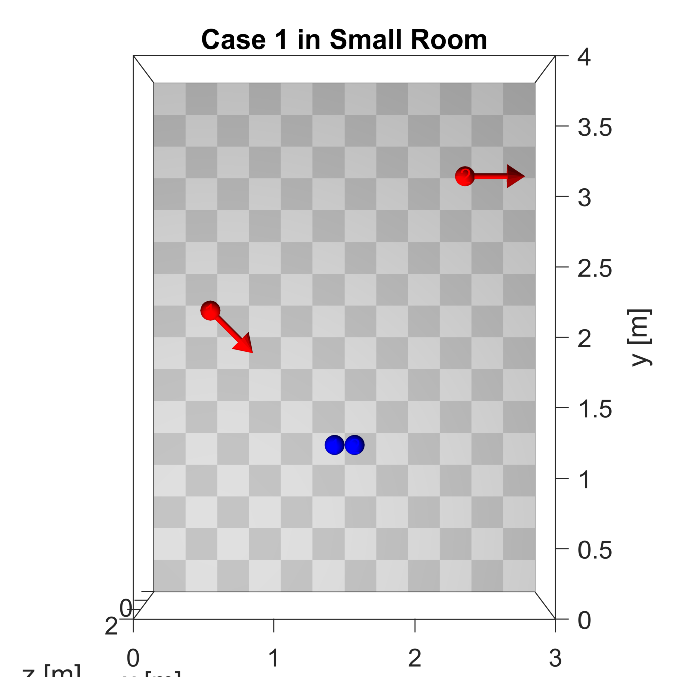
\includegraphics[width=\textwidth]{1s_lo}
\caption{Case 1}
\end{subfigure}
\begin{subfigure}[H]{0.32\textwidth}
\includegraphics[width=\textwidth]{2s_lo}
\caption{Case 2}
\end{subfigure}
\begin{subfigure}[H]{0.32\textwidth}
\includegraphics[width=\textwidth]{3s_lo}
\caption{Case 3}
\end{subfigure}
\caption{Source-Receiver Layout of Different Baseline Cases (Arrow represents the Direction of Speech)}
\label{fig:testcases}
\end{figure}
As a convention throughout the project, sources and receivers are numbered from left to right, starting from number 1. Note that speakers are labelled in red, while microphones are labelled in blue. The rationale behind setting up each baseline case is then listed.
\begin{itemize}
\item Case 1 represents scenarios where two speakers has an obvious difference in distance to the microphones. This should be reflected by the amplitude difference in the generated RIR.
\item Case 2 is a simple symmetrical case. Utilising the symmetry, the generated RIR from speaker 1 to microphone 1 would be expected be the same as the RIR from speaker 2 to microphone 2.
\item Case 3 is similar to Case 2, with the only change being the distance of the direct path from the speaker to the microphone. This should be reflected by the decrease in amplitude at the first peak as compared to Case 2.
\end{itemize}

Below collates and explains some key results obtained from the baseline cases using the acoustic model of a small room. The full results for each of the 3 baseline cases in the 3 choices of rooms are included in Appendix \ref{appendixresult}.

\begin{figure}[H]
\centering
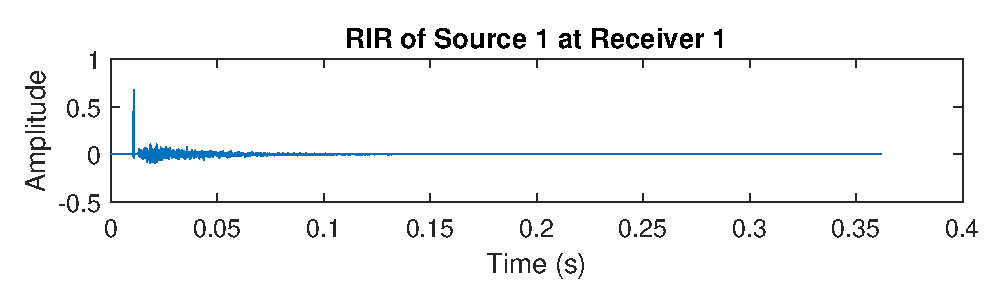
\includegraphics[width=0.8\textwidth]{c1s1r1}
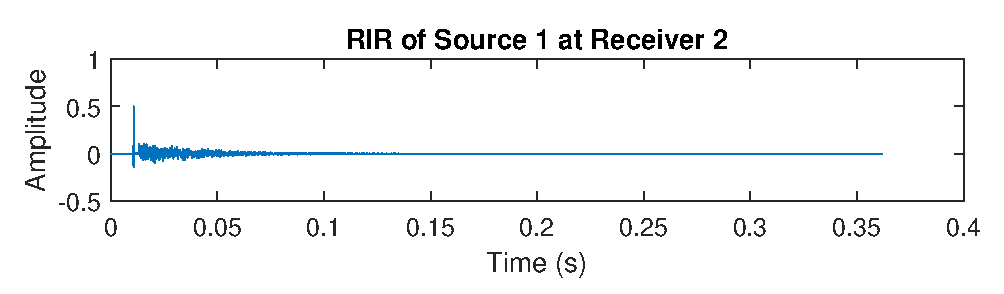
\includegraphics[width=0.8\textwidth]{c1s1r2}
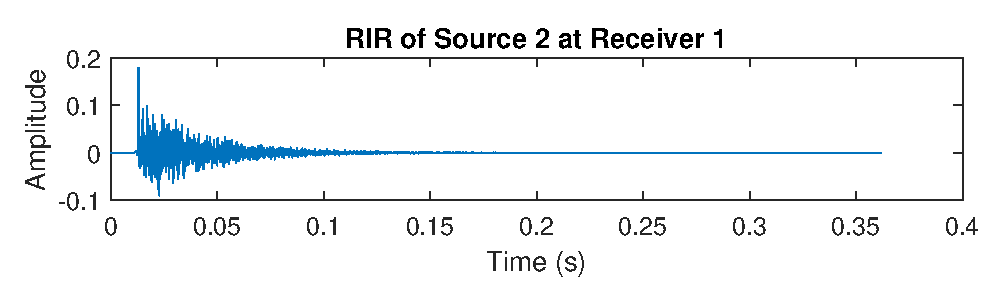
\includegraphics[width=0.8\textwidth]{c1s2r1}
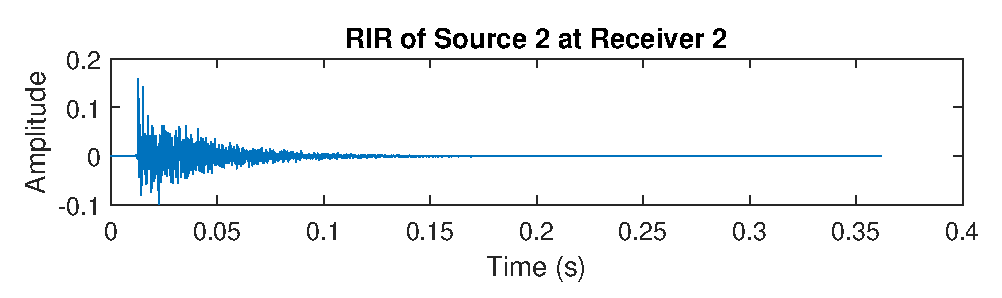
\includegraphics[width=0.8\textwidth]{c1s2r2}
\caption{Room Impulse Responses for Case 1}
\label{fig:case1}
\end{figure}

\Cref{fig:case1} shows the resulting RIR of case 1 in a small room. In the RIR, the earliest peak represents the direct path, while the later peaks corresponds to the reverberation produced by the reflected paths. It can be observed that the earliest peak of the RIR of source 1 is much higher than that of source 2, as expectedly.
\begin{figure}[H]
\centering
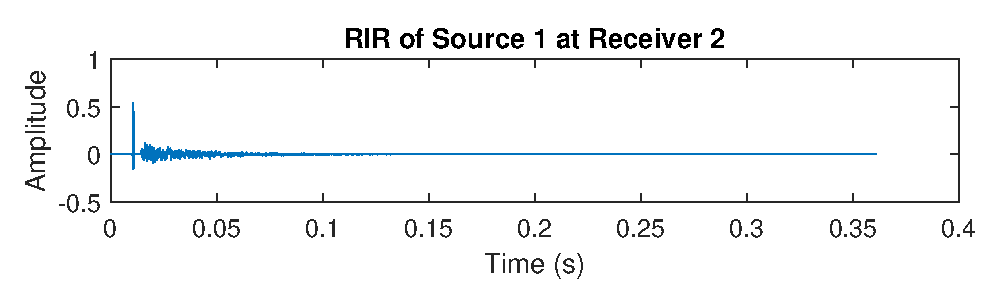
\includegraphics[width=0.8\textwidth]{c2s1r2}
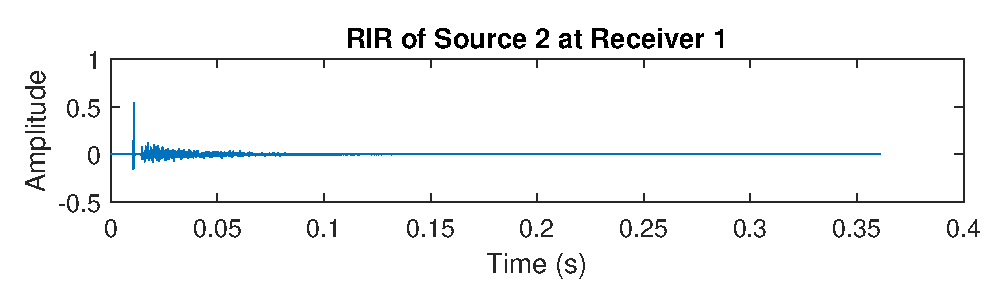
\includegraphics[width=0.8\textwidth]{c2s2r1}
\caption{Room Impulse Responses for Case 2}
\label{fig:case2}
\end{figure}
\begin{figure}[H]
\centering
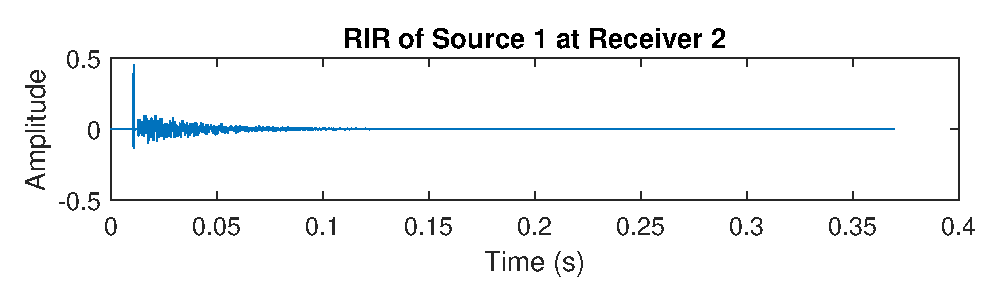
\includegraphics[width=0.8\textwidth]{c3s1r2}
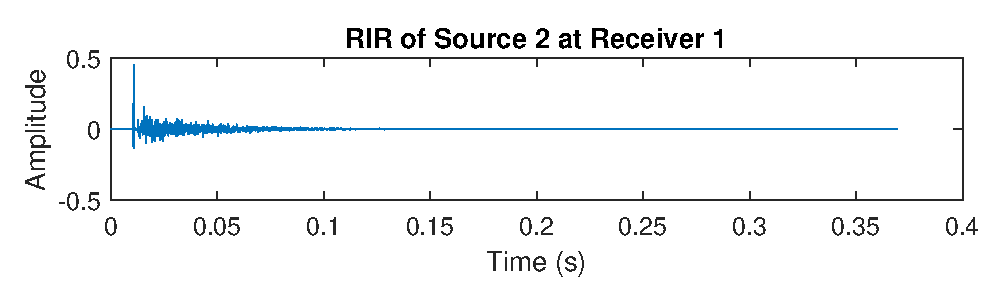
\includegraphics[width=0.8\textwidth]{c3s2r1}
\caption{Room Impulse Responses for Case 3}
\label{fig:case3}
\end{figure}
\Cref{fig:case2} shows the RIRs from case 2. Contrary to case 1, it can be seen that the RIR from Source 1 to Receiver 2 is the same as the RIR from Source 2 to Receiver 1. This verifies the hypothesis where the symmetry of the room leads to the same impulse response. \Cref{fig:case3} shows the resulting RIRs for case 3. Same as case 2, due to the symmetry of the room layout, the RIR is the same from Source 1 to Receiver 2 and from Source 2 to Receiver 1. The difference between the two cases is once again the direct-path peak. As designed, the distance from source to receiver are made larger in case 3. Hence, it can be observed that the direct path peak is lower as compared to case 2. 

Overall, by comparing different baseline cases, it has been shown that the software generates the correct RIR for specific microphone and speaker locations within a room with an arbitrary size.
\subsection{Results}
With both anechoic speech data and the software platform for generating RIR available, the final step is to combine them to simulate the synthetic echoic speeches. With the aid of spectrogram, below discusses the effect of the room acoustics towards the anechoic speeches, and displays the results of the received signal using baseline case 2 in a small room.

\begin{figure}[H]
\centering	
\begin{subfigure}[H]{0.9\textwidth}
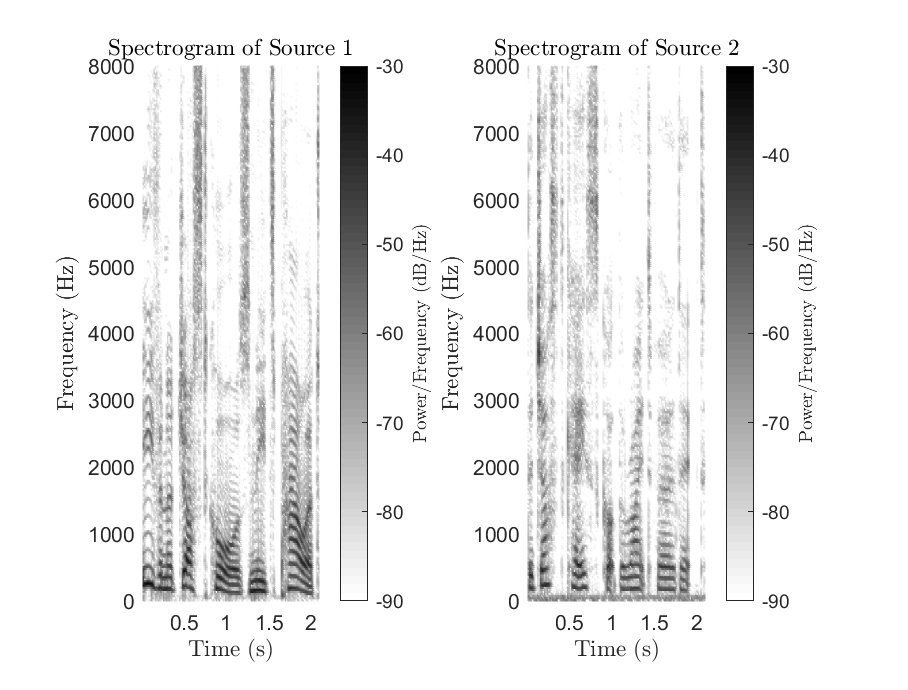
\includegraphics[width=\textwidth]{spectsrc}
\caption{Original Anechoic Speech}
\vspace*{0.5cm}
\end{subfigure}
\begin{subfigure}[H]{0.9\textwidth}
\includegraphics[width=\textwidth]{reverb}
\caption{Echoic Speech}
\end{subfigure}
\caption{Spectrograms of the Anechoic Speech and the Echoic Speech}
\label{fig:reverberatedspeech}
\end{figure}
\Cref{fig:reverberatedspeech} shows the spectrogram of the anechoic and echoic speech, generated using Hamming window of $N_w = 512$, with an overlapping factor of 2 under a sampling frequency of 16kHz. It can be observed from the spectrogram that the echoic speech gives rise to a more ``blurry'' spectrogram. This is particularly evident looking at the dark areas, which represents the formant frequencies. In anechoic speech, the formant frequencies can easily be observed, while in echoic speech, they looks submerged by the surroundings. This is mainly due to the reverberation from the reflection of the walls, which leads to a temporal ``dispersion'' of the dark areas. It hence verifies the software simulation to generate synthetic echoic audio data. \Cref{fig:spectrec} shows the resultant echoic mixture received by the microphones.

\begin{figure}[H]
\centering	
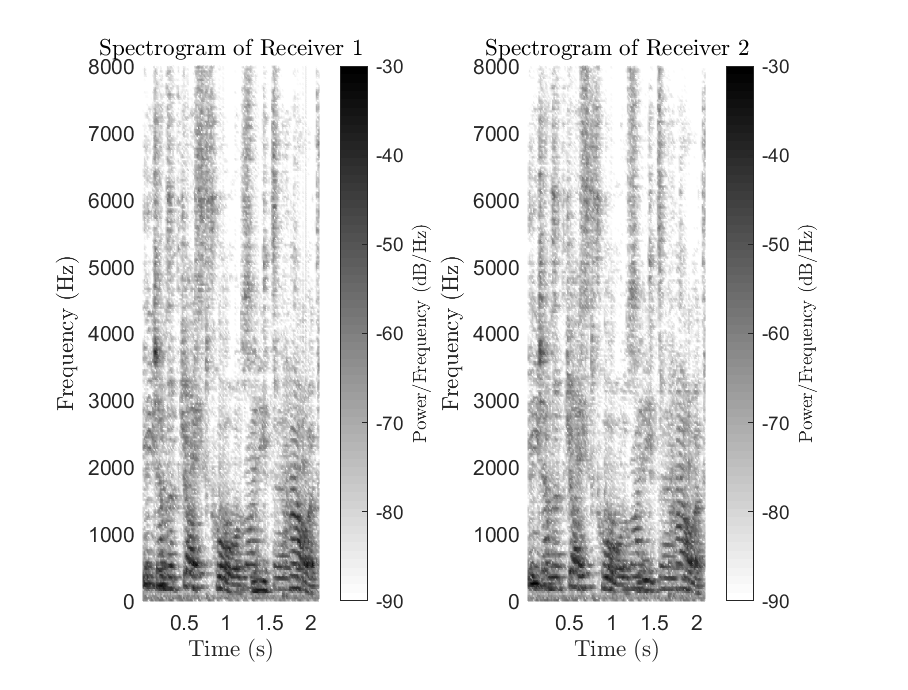
\includegraphics[width=0.9\textwidth]{spectrec}
\caption{Spectrogram of Received Mixture of Echoic Speech}
\label{fig:spectrec}
\end{figure}

\newpage
\section{Algorithmic Development}
\label{sect:phaseII}
Having built a robust software simulation platform, the next step is to develop the processing algorithm. Using the only information obtained, which is the DOA of the \textbf{desired} speaker, below proposes a few approaches, namely beamforming, time-frequency Masking through clustering and machine learning. 

\subsection{Beamforming}
\subsubsection{Motivation}
As introduced in \Cref{sect:beamformingreview}, beamforming is an established audio zooming technique typically used in large microphone arrays. Despite facing with problems such as spatial aliasing and wide beamwidth, it was still worthwhile to observe the effect of beamforming in a dual-microphone set-up, and investigate its effectiveness in the context of the project.
\subsubsection{Delay-Sum Beamformer (DSB)}
The first basic type of beamformer experimented was the delay sum beamformer. As its name suggests, it was done by simply delaying and summing. The theory is illustrated in \Cref{fig:dsb}. It can be seen that for a signal coming from a specific DOA $\theta$, it possesses a unique TDOA $\delta$. By delaying the signal by its corresponding $\delta$, constructive interference would be steered to the desired DOA. In contrast, signal coming from other DOA will be attenuated.
\begin{figure}[H]
\centering
\includegraphics[width=0.7\linewidth]{steer}
\caption{Illustration of theory of delay-sum beamformer formed of 3 microphones. (From \cite{TheLabBookPagesDelayCalculation})}
\label{fig:dsb}
\end{figure}
\paragraph{Array Pattern}
To quantify the performance provided by a beamformer, the gain across different DOA has to be found. The key in deriving the array pattern was to operate in frequency domain. 

Firstly, consider \Cref{fig:delay}, to steer the beam towards a DOA of $\hat{\theta}$, the signal received at microphone 1 has to be delayed by $\hat{\delta}=\frac{d}{c}\sin\hat{\theta}$, as derived in \Cref{eq:delay}. In frequency domain, this is equivalent to multiplying an exponential term of $e^{-j\omega\frac{d\sin\hat{\theta}}{c}}$ to the received signal at microphone 1. 

Now, consider a signal arriving with an angle $\theta$. As microphone 1 receive the same signal as microphone 2 earlier by $\delta=\frac{d}{c}\sin\theta$. This introduces a factor of $e^{j\omega\frac{d\sin\theta}{c}}$ to the received signal at microphone 1 with respect to that of microphone 2 in frequency domain.

Incorporating two factors, the gain at the microphone 1 can be expressed as
\begin{align}
H_1(\omega,\theta)=e^{-j\omega\frac{d\sin\hat{\theta}}{c}}e^{j\omega\frac{d\sin\theta}{c}}=e^{\frac{j\omega d(\sin\theta-\sin\hat{\theta})}{c}}
\end{align}
where $\hat{\theta}$ is the steering angle of the beamformer, and $\theta$ is the actual DOA of the received signal. On the other hand, as microphone 2 is the reference microphone, the gain at microphone 2 would be unity. Hence, the array pattern is given by 
\begin{align}
H(\omega,\theta)=\frac{1}{2}(H_1(\omega,\theta)+H_2(\omega,\theta))=\frac{1}{2}\left(e^{\frac{j\omega d(\sin\theta-\sin\hat{\theta})}{c}}+1\right)
\end{align}
where the factor of $\frac{1}{2}$ is to normalise the array pattern to have a maximum gain of unity. This deduction has been summarised in \Cref{fig:dsbblock}.

\begin{figure}[H]
\centering
\includegraphics[width=\linewidth]{dsbblockdiagram}
\caption{Block Diagram of a dual-microphone beamformer in frequency domain}
\label{fig:dsbblock}
\end{figure}

Observing the expression for array pattern, it can be seen that constructive interference ($|H(\omega,\theta)|=1$) occurs when $\theta=\hat{\theta}$, which means when the steering angle is the same as the DOA of the received signal. 

\paragraph{Results}
A simple example would be using \textbf{baseline case 2} in \Cref{fig:testcases}, where the DOA of desired speaker is $\theta_1 = 45^\circ$, and the DOA of the interfering speaker is $\theta_2 = -45^\circ$. To begin with, the microphone separation was set to be 10cm, complying with the usual microphone set-up in mobile phones. 

For visualisation, the array pattern are plotted for different frequencies in the voice band, which ranges from 300Hz to 3400Hz \cite{Freeman2005FundamentalsTelecommunications}. In telephony, the voice band represents the harmonic series of human fundamental frequency that are required for the speech to be audible. Hence, by observing the array pattern within the voice band, the behaviour of the beamformer towards speech could be known.

\begin{figure}[H]
\centering
\includegraphics[width=0.3\linewidth]{dsbd10f300}
\includegraphics[width=0.3\linewidth]{dsbd10f500}
\includegraphics[width=0.3\linewidth]{dsbd10f1000}
\includegraphics[width=0.3\linewidth]{dsbd10f1700}
\includegraphics[width=0.3\linewidth]{dsbd10f2500}
\includegraphics[width=0.3\linewidth]{dsbd10f3000}
\caption{Array Pattern of Delay Sum Beamformer for frequency range 300-3000 Hz}
\label{fig:dsbpattern}
\end{figure}

\Cref{fig:dsbpattern} shows the array pattern when the beam angle is $45^\circ$ and the separation of microphones $d$ is 10cm. From the figure, all array patterns contain unity response at $45^\circ$, which verifies the software implementation. Following the discussion in \Cref{sect:beamformingreview}, a trade off between spatial selectivity and spatial aliasing has also been shown. At low frequencies, the beam width of the beamformer is very large, due to the fact that the $\frac{d}{\lambda}$ is small, as given in \Cref{eq:beamwidth}. At $f=1700$Hz, $d=\frac{\lambda}{2}$, which is the maximum separation without spatial aliasing. For higher frequencies, as $d>\frac{\lambda}{2}$, despite a narrow beam width, spatial aliasing was observed, where multiple beams evolved.

This result shows that the choice of the microphone separation directly affects the filtering effect across frequencies. Below attempts to vary the microphone separations and evaluate using the Source-to-Interference Ratio (SIR) under free field and reverberant environment. As the change of microphone position leading to slight differences in the SIR value, to allow a fair ground for comparison, instead of the absolute value, the gain in SIR was instead shown. This was defined as
\begin{align}
\text{SIR}_\text{gain} = \text{SIR}_\text{zoomed}-\text{SIR}_\text{unprocessed} \label{eq:SNRgain}
\end{align}
in dB, which shows the extent of improvement that beamforming performed as an audio zooming technique. 

\begin{table}[H]
\centering
\begin{tabularx}{0.75\textwidth}{|l|Y|Y|Y|Y|}
\hline
$\text{SIR}_\text{gain}$ (dB) & $d=$2cm & $d=$5cm & $d=$10cm & $d=$15cm \\ \hline
RT$_{60}$=0ms & 0.4839 & 0.5981 & 1.3111 & 2.3992 \\ \hline
RT$_{60}$=200ms & 0.1203 & 0.5342 & 1.5438 & 2.1183 \\ \hline
RT$_{60}$=400ms & 0.1310 & 0.8107 & 1.2954 & 1.0766 \\ \hline
\end{tabularx}
\caption{Performance of Delay Sum Beamformer under different degree of reverberation}
\label{table:delaysumperformance}
\end{table}

\Cref{table:delaysumperformance} shows the results by varying the separation in range of 2cm to 15cm, fulfilling the dimension restriction of a mobile phone. From the SIRs, it can be seen that the zooming effect is most significant when $d=15$cm, achieving a gain in SIR of 2.4 dB. Also, the results verified that the degrading of performance of DSB encountering reverberation. This was expected as reflected paths meant that some of the reflected paths from interfering signal may have the same DOA as the direct path of the desired source.

\subsubsection{Linear Constraint Minimum Variance (LCMV) Beamformer}
\label{sect:adaptivebeamformer}
However, observing from the beam patterns, the only aim of DSB was to keep the signal of interest. However, in the context of audio zooming, suppression of interfering source is also very important. This gave rise to  adaptive beamforming, where the beamformer utilizes the information from the received signal to maximize the received signal power while minimizing interfering noise. One example is the LCMV beamformer, which aims to minimize the total output power of an array subject to some constraints. Consider the case where the constraints are to maintain the signals coming from specific DOAs, then LCMV beamformer effectively becomes an interference canceller. Below formulates the problem mathematically.

\paragraph{Problem Formulation}
Extending the usage of DSB in frequency domain, beamforming can be done by applying a complex weight to each sensor and summing across all sensor \cite{Habets2009OnEnhancement}. 
\begin{align}
y=\textbf{w}^H\textbf{x}
\end{align}
where $y$ is the output signal, and $\textbf{x}=[x_1,...,x_N]^T$ is the column vector containing the signals received at all $N$ sensors. The output power of the beamformer is then given by
\begin{align}
P = \mathcal{E}\{y^Hy\}=\mathcal{E}\{\textbf{w}^H\textbf{x}^H\textbf{x}\textbf{w}\}=\textbf{w}^HR_{xx}\textbf{w}
\end{align}
where $\mathcal{E}\{\cdot\}$ denotes expectation, and $R_{xx}=\mathcal{E}\{\textbf{x}\textbf{x}^H\}$ is the covariance matrix of \textbf{x}.

For the constraint, every direction $(\theta,\phi)$ has a corresponding steering vector, $\textbf{c}(\theta,\phi)$, which performs the same effect as delaying in time domain. The response of the array to the steering vector is given by $\textbf{c}(\theta,\phi)^H\textbf{w}$. Therefore, the constraints can now be written as
\begin{align}
\textbf{c}(\theta,\phi)^H\textbf{w}=q
\end{align}
where $q$ is the desired response value. 

The LCMV problem can then be formulated as
\begin{align}
\min_\textbf{w} \textbf{w}^HR_{xx}\textbf{w} \, \text{ subject to } C^H\textbf{w}=\textbf{q} \label{eq:LCMV}
\end{align}
where C and \textbf{q} are formed by collating the constraints into columns.

The solution of \Cref{eq:LCMV} is then given in \cite{benesty2008microphone} as 
\begin{align}
\textbf{w}_\text{LCMV}=R_{xx}^{-1}C(C^HR_{xx}^{-1}C)^{-1}\textbf{q} \label{eq:solutionLCMV}
\end{align}
An interesting point is that the maximum number of constraints. As seen from \Cref{eq:solutionLCMV}, solution only exists when $C^HR_{xx}^{-1}C$ is invertible. Hence, it can be seen that the number of constraints should not exceed the number of microphones. This solved a constrained optimisation problem, and allow the beamformer to specify its desired response at a certain angle. 

\paragraph{Minimum Variance Distortionless Response (MVDR) Beamformer}
Minimum Variance Distortionless Response (MVDR) Beamformer is a special type of the LCMV beamformer with only one constraint \cite{Habets2009OnEnhancement} that the signal coming from a certain angle $(\theta,\phi)$ is distortionless. By distortionless, it means that the desired response $q=1$. With only one constraint, one could easily rewrite the LCMV solution as
\begin{align}
\textbf{w}_\text{MVDR}=\frac{R_{xx}^{-1}\textbf{c}(\theta,\phi)}{\textbf{c}^H(\theta,\phi)R_{xx}^{-1}\textbf{c}(\theta,\phi)}
\end{align}
This result was particularly useful in this project, as the solution only requires the spatial information of the desired user. Using this solution, the same experiment as DSB was done again with $\theta_1=45^\circ,\theta_2 = -45^\circ,d=10$cm. The constraint imposed was $\textbf{c}^H(45^\circ,0^\circ)\textbf{w}=1$, and the results are shown in \Cref{fig:mvdrpattern}.
\begin{figure}[H]
\centering
\includegraphics[width=0.3\linewidth]{mvdrd10f300}
\includegraphics[width=0.3\linewidth]{mvdrd10f500}
\includegraphics[width=0.3\linewidth]{mvdrd10f1000}
\includegraphics[width=0.3\linewidth]{mvdrd10f1700}
\includegraphics[width=0.3\linewidth]{mvdrd10f2500}
\includegraphics[width=0.3\linewidth]{mvdrd10f3000}
\caption{Array Pattern of MVDR Beamformer for frequency range 300-3000 Hz}
\label{fig:mvdrpattern}
\end{figure}

It can be seen that the array pattern at $\theta_1=45^\circ$ is always kept at 1 as expected by the imposed constraint. However, one drawback of the algorithm is that initialisation is required to estimate the noise signal. This could be seen by observing from the pattern without initialisation in \Cref{fig:mvdrpattern}, where a null was inserted across all frequencies at azimuth of $0^\circ$ at the wrong DOA. Unfornately, due to time constraint, this problem was not solved. Despite erroneous localisation, MVDR beamformer has demonstrated its power to cancel interferences. 

\paragraph{Generalised Sidelobe Canceller (GSC)}
As a commonly used beamformer, generalized sidelobe canceller (GSC) \cite{Griffiths1982AnBeamforming} is another example of an adaptive beamformer. As seen from \Cref{fig:gsc}, it consists of a delay-sum beamformer (top branch) and a tapped delay line (bottom branch). The top branch performs the same as a conventional beamformer to provide constructive interference to the wanted signals at a certain DOA. Contrarily, the bottom branch aims to model the interference by passing the signal firstly into the blocking matrix, which is orthogonal and removes the signal of interest, and then filtered by a bank of FIR filters. The adaptive weights of the FIR filters are updated using least mean-square (LMS) algorithm. The difference between two branches would then form the output of the GSC.

Besides, GSC is actually an efficient implementation of a LCMV beamformer. As seen from \Cref{eq:solutionLCMV}, the solution requires matrix inversion, which is computationally expensive. GSC effectively transformed this constrained problem to an unconstrained problem, which simplifies the implementation. However, as the scope of the project focuses on the use of small microphone arrays, matrix inversion would be of a small size. Hence, LCMV beamformer was still preferred over GSC for its accuracy in interference suppression. The implementation of GSC has been included in \Cref{sect:beamformingcode}.

\begin{figure}[H]
\centering
\captionsetup{justification=centering}
\includegraphics[width=0.7\textwidth]{gsc_signal_flow}
\caption{Block Diagram of the Generalised Sidelobe Canceller (From \cite{Griffiths1982AnBeamforming})}
\label{fig:gsc}
\end{figure}

\subsubsection{Summary}
In this section, different techniques of beamforming was attempted. Despite demonstrating a weak audio zooming effect, it demonstrated the ability to localise and nullify interferences. Hence, it could be served as an enhancement technique, coupled with other audio zooming techniques to produce a better result.

\subsection{Time-frequency Mask Estimation through Clustering of Phase Differences}
\label{sect:TFMask}
\subsubsection{Motivation}
With \cite{JourjineBlindMixtures} stating that there exist a perfect binary TF mask to separate speech signals, an estimation technique to form the TF mask is thought to be a way forward. Hence, the first approach attempted is forming TF mask to ``extract'' the desired speech signal. Throughout the project, it is emphasised that the only information in hand is the DOA of the desired human speaker. The problem now remains to translate this information into parameters that can be obtained in TF domain.

Revisiting the \Cref{sect:beamformingreview} about delay calculation in beamforming, it is shown that signal coming from different DOA $\theta$ results in different delays $\delta$ between the received signal by the microphones. Using the relationship given by \Cref{eq:delay}, DOA can be translated into TDOA, which effectively transformed a spatial parameter into a temporal parameter. 

With the TDOA of the desired speaker now available, the next step is to relate it with the TF representation of the received signals. This can be done using the \textbf{narrowband assumption} given by \Cref{eq1}, which states that when the separation of the microphones is sufficiently small, time delay $\delta$ of the signal can be translated into a phase shift of $-\omega\delta$ in the TF domain. Further to that, from the \textbf{W-disjoint orthogonality assumption}, each TF bin will only be occupied by one of the speakers. In other words, the phase difference between received signals at microphone 1 and 2 at each TF bin can be assigned to an unique speaker.

To formally represent this, firstly define the short-time cross power spectral density $G_{12}(\tau,\omega)$ of received signal $x_1(t)$ and $x_2(t)$ as 
\begin{align}
G_{12}(\tau,\omega) = (X^W_1(\tau,\omega))^*X^W_2(\tau,\omega)
\end{align}
where $X^W_k(\tau,\omega)$ refers to the STFT of received signal at $k$-th microphone. The phase difference between received signals at microphone 1 and 2 can then be defined as the phase of the cross power spectral density using
\begin{align}
\phi_{12}(\tau,\omega) = \angle G_{12}(\tau,\omega).
\end{align}
From the above deduction using the \textbf{narrowband assumption} and \textbf{W-disjoint orthogonality assumption}, $\phi_{12}$ can be represented by
\begin{align}
\phi_{12}(\tau,\omega) = -\omega\delta_j \label{eq:phasediff}
\end{align}
where $\delta_j$ is TDOA of the speech signal $s_j(t)$ that occupies the TF bin. Therefore, using the phase difference between received signals of microphones, one can effectively decide if the TF bin belongs to the desired speech signal coming from a known DOA. This classification or assignment of membership is called TF masking. By applying this TF mask onto the mixture of signals, the desired speech signal can then be retrieved. 

\subsubsection{Baseline Testing using Naive Binary Mask}
To begin with, the time representation of the signal has to be transformed into a TF representation. Under the help of \texttt{VOICEBOX} \cite{Brookes1997VOICEBOX:MATLAB.}, particularly with the routines \texttt{enframe.m}, the signal is split into overlapping frames. In this time-frequency analysis, the simulated audio signal received by the two microphones is first split into time frames using Hamming window of $N_w = 512$, with an overlapping factor of 2 under sampling frequency of 16kHz. In other words, the signals has been split into overlapping time-frame of $t=\frac{512}{16000}=32$ms. After TF Masking, the TF representation would be transformed back to the time-domain signal using overlap-add method using \texttt{overlapadd.m}. As the signal is now represented in discrete time and discrete frequency, the phase difference is now instead represented by 
\begin{align}
\varphi(k,l)=\phi_{12}(k\tau_0,l\omega_0)
\end{align}
where $\tau_0$ and $\omega_0$ are the corresponding time and frequency resolution. In this case, $\tau_0=\frac{256}{16000}=16\text{ms}$, and $\omega_0=2\pi\frac{16000}{512}=62.5\pi\text{rad/s}$

To verify the feasibility of the proposed approach, as well as the validity of the derivation above, the first step is to develop a ``naive'' binary mask using phase difference in \textbf{free field}.

A simple example would be again using \textbf{baseline case 2} in \Cref{fig:testcases}, where the DOA of desired speaker is $\theta_1 = 45^\circ$, and the DOA of the interfering speaker is $\theta_2 = -45^\circ$. With this information, a crude ``naive'' decision could be made based on the sign of the phase difference as stated below.
\begin{align}
M(k,l) = \begin{cases} 1, & \text{if } \varphi(k,l)<0 \\ 0, & \text{otherwise} \end{cases} \label{eq:naivemask}
\end{align}
\paragraph{Separation of Microphone $d$}
One problem faced by this approach is the phase wrapping. Revisiting \Cref{eq:phasediff}, the phase difference can be represented as $-\omega\delta_j$. However, when $|\omega\delta_j|>\pi$, the received phase difference $\phi_{12}(\tau,\omega)$ would be a wrapped version of $-\omega\delta_j$, lying in the principal range of $(-\pi,\pi]$. This wrapping can be defined as 
\begin{align}
\varphi(k,l)=(-l\omega_0\delta_j+\pi)\text{ mod }2\pi -\pi
\end{align}
To avoid this ambiguity, $|l\omega_0\delta_j|<\pi$ has to be satisfied for all TF points $(k,l)$. Hence, the equation can be rewritten as 
\begin{align}
\omega_\text{max}\delta_\text{max}<\pi
\end{align}
where $\omega_\text{max}$ is the maximum frequency of interest and $\delta_\text{max}$ is the maximum possible TDOA. As discussed in \Cref{eq:delay}, $\delta_\text{max}=\frac{d}{c}$. Hence, this relation can again be rewritten as
\begin{align}
d < \frac{c\pi}{\omega_\text{max}}.
\end{align}
Here, the design choice became to choose $\omega_\text{max}$. For a full band implementation, $\omega_\text{max}=\pi f_s$, where $f_s$ is the sampling frequency of the speech signal. Therefore, with a sampling frequency of 16kHz, the maximum distance between the microphones would be $d\approx\frac{340}{16000}=2.125\text{cm}$. This restriction could potentially be further reduced if $\omega_\text{max}<\pi f_s$. In the context of this project, the human voice frequency is considered. In telephony, the voice band ranges from 300Hz to 3400Hz \cite{Freeman2005FundamentalsTelecommunications}. Using this as a reference, the maximum microphone separation without a significant impairment to the speech signal is $d\approx\frac{340\pi}{2\pi3400}=5\text{cm}$. 

\Cref{fig:phasediffspec} then visualises the discussion. At $d=2\text{cm}$, no phase wrapping occurs. Hence, it can be easily observed that the green regions belongs to the desired user. However, at $d=5\text{cm}$, phase wrapping happens at high frequency regions beyond 3400Hz. When the separation is too large, at $d=15\text{cm}$, it is obvious that phase wrapping has a significant impact by observing the strong red and cyan horizontal regions in the spectrogram. 

In this algorithmic development stage, $d=2\text{cm}$ is used for a complete evaluation of the performance of the algorithm. However, it is well noted that in smartphones, a separation of 5cm would a more feasible solution to the problem.
\begin{figure}[H]
\centering	
\begin{subfigure}[H]{0.49\textwidth}
\includegraphics[width=\textwidth]{phasediffspectd2}
\caption{$d=2\text{cm}$}
\end{subfigure}
\begin{subfigure}[H]{0.49\textwidth}
\includegraphics[width=\textwidth]{phasediffspectd5}
\caption{$d=5\text{cm}$}
\end{subfigure}
\\[1em]
\begin{subfigure}[H]{0.49\textwidth}
\includegraphics[width=\textwidth]{phasediffspectd15}
\caption{$d=15\text{cm}$}
\end{subfigure}
\caption{Phase Difference $\varphi(k,l)$ under different microphone separation}
\label{fig:phasediffspec}
\end{figure}

\paragraph{Results}
Results of the formed binary mask is then shown in \Cref{fig:speccomp}. It can be observed that the proposed naive TF binary mask successfully labels most TF bins from speaker 1 and retrieves the speech signal. It verifies the feasibility of using TF masks to perform audio zooming.
\begin{figure}[H]
\centering	
\begin{subfigure}[H]{0.49\textwidth}
\includegraphics[width=\textwidth]{spectsrc1}
\caption{Anechoic Speech}
\end{subfigure}
\begin{subfigure}[H]{0.49\textwidth}
\includegraphics[width=\textwidth]{naivemask1}
\caption{Naive Binary Mask}
\end{subfigure}
\\[1em]
\begin{subfigure}[H]{0.49\textwidth}
\includegraphics[width=\textwidth]{spectnaive1}
\caption{Zoomed Speech}
\end{subfigure}
\caption{Evaluating the performance of TF mask in free field}
\label{fig:speccomp}
\end{figure}

Despite a successful demonstration of theory, the naive binary mask still had some major questions to answer. The major question was that in the development of the binary mask, the DOA of the interfering source was assumed to be known. However, in the context of this project, only the DOA of the desired speaker was assumed to be known. Therefore, it gave rise to the need of localising the interfering sources and getting the DOA of the interfering sources. 
\subsubsection{$k$-means Clustering}
To achieve that, clustering techniques are introduced. The first clustering technique is an iterative process named $k$-means clustering \cite{Hartigan1979}. The objective of $k$-means clustering is to partition the $n$ samples into $k$ sets as to minimize the within-cluster euclidean distances, defined as
\begin{align}
J_\text{$k$-means} =\sum _{i=1}^{k}\sum _{\mathbf {x} \in S_{i}}\left\|\mathbf{x} -{\boldsymbol {\mu }}_{i}\right\|^{2} \label{eq:objkmeans}
\end{align}
where $\mathbf{x}$ is the data point, $S_i$ is the set representing $i$-th cluster, and ${\boldsymbol {\mu }}_{i}$ is the centroid of the $i$-th cluster. In the context of this report, $k$ refers to the number of speakers in total, which is 2.

\paragraph{Data Formulation}
Before clustering, a consideration should be made on how to formulate the data in a way that TF bins belonging to the same speaker has a similar data value. Again, the TDOA value could be used. This could be derived from \Cref{eq:phasediff} as 
\begin{align}
\hat{\delta}(k,l)=\frac{-\varphi(k,l)}{l\omega_0}.
\end{align}
By representing this each TF bin in this form and collating this feature into a vector, the data is now ready for clustering. 

\paragraph{Forming the clusters}
The next step was to form the clusters. $k$-means clustering adopts an iterative process, consisting of initialisation, assignment and updating.

Firstly, the data were partitioned randomly as an initialisation step. Centroids were then computed for each cluster. Comparing the Euclidean distances to each centroid, the data point was then assigned to the nearest cluster. This assignment and update process repeated until the change of objective function stated in \Cref{eq:objkmeans} was smaller than an arbitrarily small value $\epsilon$, which concludes the clustering process.

\paragraph{Cluster Labelling}
Forming the clusters, the remaining step was to find out which clusters belong to the desired speaker. This was achieved by again comparing the distance from the known TDOA $\delta$ of the desired speaker to that of each centroid and choosing the minimum. 

\paragraph{Result}
With the features formulated and number of clusters decided, the resultant mask is then displayed in \Cref{fig:maskkmeans}.
\begin{figure}[H]
\centering
\begin{subfigure}[H]{0.49\textwidth}
\includegraphics[width=\textwidth]{naivemask1}
\caption{Naive Binary Mask}
\end{subfigure}
\begin{subfigure}[H]{0.49\textwidth}
\includegraphics[width=\textwidth]{maskkmeans}
\caption{$k$-means clustering}
\end{subfigure}
\caption{Comparison of ``Naive'' Binary Mask and $k$-means Clustering}
\label{fig:maskkmeans}
\end{figure}
Comparing the two binary masks, it can be seen that both methods produced similar results, which shows that $k$-means clustering successfully localised the interfering source as hypothesised.

\subsubsection{Soft mask using Fuzzy $c$-means Clustering (FCM)}
In the development above, the W-disjoint orthogonality assumption was considered true, which means that a TF bin can only be occupied by one source at a time. However, as depicted in \Cref{fig:wortho}, the behaviour of speech signals was found to be \textbf{approximately} W-disjoint orthogonal. In other words, a TF bin may be occupied simultaneously by multiple sources. This led to the thought of developing a soft mask using fuzzy $c$-means Clustering (FCM) \cite{Bezdek1981ObjectiveClustering}.

Compared with $k$-means clustering, the main difference is that a data point could simultaneously belong to multiple clusters in FCM. Instead of assigning each point a cluster, a membership index $0\leq u_n\leq 1$ is given to each TF point to indicate the degree of it belong to the $n$-th cluster, defined as
\begin{align}
u_{n}(\mathbf{x})=\frac{1}{\sum_{k=1}^{c}\left(\frac{\left\|\mathbf{x}-\boldsymbol{\mu}_{n}\right\|}{\left\|\mathbf{x}-\boldsymbol{\mu}_{k}\right\|}\right)}.
\end{align}
It can be seen that, the closer the data point is towards the centroid of the $n$-th cluster, the higher membership value is given as expected. Then, the formal definition of FCM is defined as an optimisation problem that aims to minimize
\begin{align}
J_\text{FCM} =\sum _{k=1}^{c}\sum_{\forall\mathbf{x}}u_k^2(\mathbf{x})\left\|\mathbf{x} -{\boldsymbol{\mu}}_{k}\right\|^{2} \label{eq:objFCM}
\end{align}
subject to $\sum_{k=1}^c u_k(\mathbf{x}) =1 \,\forall \mathbf{x}$. Again, $\mathbf{x}$ represents the data point, $c$ represents the number of clusters and $\boldsymbol{\mu}_k$ represents the centroid of the $k$-th cluster. However, as now a single point can belong to various clusters, the centroid of the cluster is redefined as a weighted mean of all data points given by 
\begin{align}
\boldsymbol{\mu}_n = \frac{\sum_{\forall \mathbf{x}} u_n(\mathbf{x})\mathbf{x}}{\sum_{\forall \mathbf{x}} u_n(\mathbf{x})} \label{eq:mufcm}
\end{align}
Similar to $k$-means clustering, by setting a threshold on the change of the objective function $J_\text{FCM}$ and iterates, the optimal clusters would be found.

\paragraph{Results}

\begin{figure}[H]
\centering
\begin{subfigure}[H]{0.49\textwidth}
\includegraphics[width=\textwidth]{maskkmeans}
\caption{$k$-means clustering}
\end{subfigure}
\begin{subfigure}[H]{0.49\textwidth}
\includegraphics[width=\textwidth]{maskFCM}
\caption{FCM}
\end{subfigure}
\caption{Comparison of $k$-means and fuzzy $c$-means clustering}
\label{fig:maskfcm}
\end{figure}
Experiment was again performed in free field, and the resultant mask is shown in \Cref{fig:maskfcm}. However, by judging on the appearance of the TF mask, no obvious conclusion could be drawn. Hence, using the evaluation metrics discussed in \Cref{sect:evaltec}, the performance was compared and listed in \Cref{table:performancecluster}.

\begin{table}[H]
\centering
\begin{tabularx}{\textwidth}{|l|l|Y|Y|Y|Y|}
\hline
Aspect & Metrics & Mixture & Naive & $k$-means & FCM \\ \hline
\multirow{2}{*}{Speech Quality} & SIR (dB) & -2.0410 & 21.3404 & 21.2588 & 21.2719 \\ \cline{2-6} 
 & MOS-LQO & 1.4601 & 2.6858 & 2.6905 & \textbf{3.1584} \\ \hline
Speech Intelligibility & STOI & 0.6104 & 0.8217 & 0.8237 & 0.8356 \\ \hline
\end{tabularx}
\caption{Performance of different clustering techniques in free field}
\label{table:performancecluster}
\end{table}

From the objective metrics, it can be seen that the clustering algorithms has successfully achieved the target of improving speech quality and intelligibility. Overall, SIR improved by around 23dB, which was an exciting result. However, focusing on the MOS-LQO score obtained from PESQ evaluation, FCM outperformed $k$-means clustering by around 0.45. This hence showed that a soft TF mask had the potential to produce high speech quality, hence, further investigation was required.

With the promising result of FCM in free field, the next step is to experiment with reverberant environment. FCM is then implemented in a simulated small room in \Cref{table:roomsize}. The RT$_{60}$ value was set to be 200ms. The resulting time-frequency mask is then shown in \Cref{fig:maskfail}.

\begin{figure}[H]
\centering
\includegraphics[width=0.49\textwidth]{maskfail}
\caption{Time-frequency Mask by FCM with RT$_{60}=200$ms}
\label{fig:maskfail}
\end{figure}

As seen from the figure, the TF mask was erroneous, which means that FCM was not robust in reverberant environment. To explain this situation, the distribution of DOA $\varphi$ has been plotted in \Cref{fig:doahist}. It can be seen that with no reverberation, there exists two clear peaks at the source DOA. However, when RT$_{60}=200$ms, the peaks are hardly observed. The reason is that the with reverberation, there exists reflective paths, which leads to different DOA values. This effectively ``flattens'' the distribution, which made clustering a more difficult task. 

\begin{figure}[H]
\centering
\begin{subfigure}[H]{0.49\textwidth}
\includegraphics[width=\textwidth]{doahistr0}
\caption{RT$_{60}=0\text{ms}$ (Free field)}
\end{subfigure}
\begin{subfigure}[H]{0.49\textwidth}
\includegraphics[width=\textwidth]{doahistr200}
\caption{RT$_{60}=200\text{ms}$}
\end{subfigure}
\caption{Histogram showing distribution of DOA with $\theta_1=-45^\circ, \theta_2=45^\circ$ under different reverberant conditions}
\label{fig:doahist}
\end{figure}

\subsubsection{Weighted Fuzzy $c$-means Clustering (wFCM)}
With the inability of FCM to deal with reverberation, one of the proposed methods for improvement was to provide a confidence weighting to each TF bin. It meant that the clustering process would cope more towards those confident TF bins. The new objective function could be written as
\begin{align}
J_\text{wFCM} =\sum _{k=1}^{c}\sum_{\forall\mathbf{x}}u_k^2(\mathbf{x})w(\textbf{x})\left\|\mathbf{x} -{\boldsymbol{\mu}}_{k}\right\|^{2}.
\end{align}
The centroid ${\boldsymbol{\mu}}_{k}$ is calculated by
\begin{align}
\boldsymbol{\mu}_n = \frac{\sum_{\forall \mathbf{x}} u_n(\mathbf{x})w(\textbf{x})\mathbf{x}}{\sum_{\forall \mathbf{x}} u_n(\mathbf{x})w(\textbf{x})}.
\end{align}
The update of $u_n(\mathbf{x})$ is the same as that of FCM, as shown in \Cref{eq:mufcm}. Note that when $w(\textbf{x})=1 \,\forall \textbf{x}$, wFCM defaults to FCM. Below investigates the candidate of weighting factor.

\paragraph{Variance}
One of the weighting measure was introduced by \cite{kuhnerobust}, which assumed that TF regions with low fluctuations of $\hat{\delta}(k,l)$ are not affected by reflections, possess high SNR, and only belongs to one source. To quantify this fluctuations, local variance was introduced as
\begin{align}
\sigma^2(k,l) = \frac{1}{|N|-1} \sum_{\forall(k',l')\in N}[\hat{\delta}(k',l')-\mu_{\hat{\delta}}(k,l)]^2
\end{align}
where $\mu_{\hat{\delta}}(k,l)$ is the local mean defined by
\begin{align}
\mu_{\hat{\delta}}(k,l) = \frac{1}{|N|}\sum_{\forall(k',l')\in N}\hat{\delta}(k',l').
\end{align}
Here, $N$ represents the time-frequency window selected. Using this result, the weight at TF bin $(k,l)$ can be written as
\begin{align}
w(k,l)=1+\frac{1}{\max(\sigma^2(k,l),\kappa)}
\end{align}
where $\kappa$ controls the upper limit of the weight. From this relationship, it can be seen that when the variance is low, the weights assigned would be high, indicating the TF bin is most likely reliable. As suggested by \cite{kuhnerobust}, the value of $\kappa$ was set to be $10^{-3}$, and $N$ was set to be a 11-point window of neighbouring TF bins.

\paragraph{Signal-to-Noise Ratio (SNR)}
An alternative measure would be using the Signal-to-Noise Ratio at each TF bin. This was proposed with the rationale that, when the SNR is high at a particular TF bin, it would be more likely for the TF bin to provide a reliable phase value.

\begin{figure}[H]
\centering
\includegraphics[width=0.49\textwidth]{snrspect}
\caption{SNR at each Time-frequency point}
\end{figure}
The weights are then give by
\begin{align}
w(k,l)=\min\{\text{SNR}(k,l),\kappa\}
\end{align}
where $\kappa$ again controls the upper limit. In this report, the value used is $\kappa=100$dB.

\paragraph{Results}
Using both candidate weighting scheme to form the weights, the results are then shown below in \Cref{fig:wfcm}. 

\begin{figure}[H]
\centering
\begin{subfigure}[H]{0.49\textwidth}
\includegraphics[width=\textwidth]{maskwFCM}
\caption{Variance weighted}
\end{subfigure}
\begin{subfigure}[H]{0.49\textwidth}
\includegraphics[width=\textwidth]{maskwFCM_SNR_}
\caption{SNR weighted}
\end{subfigure}
\caption{Time-frequency Mask generated using wFCM}
\label{fig:wfcm}
\end{figure}
As there was no obvious difference in the TF mask, the performance is then evaluated in \Cref{table:wFCM}. This shows that both of the proposed weightings provided similar performance, while SNR provides a slightly better interference suppression.
\begin{table}[H]
\centering
\begin{tabularx}{0.9\textwidth}{|l|l|Y|Y|Y|}
\hline
Aspect & Metrics & Mixture & Variance & SNR \\ \hline
\multirow{2}{*}{Speech Quality} & SIR (dB) & -2.2494 & 0.8102 & \textbf{0.8923}  \\ \cline{2-5} 
 & MOS-LQO & 1.4260 & 1.5175 & 1.5214 \\ \hline
Speech Intelligibility & STOI & 0.5728 & 0.6176 & 0.6198 \\ \hline
\end{tabularx}
\caption{Performance of wFCM in RT$_{60}=200$ms}
\label{table:wFCM}
\end{table}

\subsubsection{Weighted Contextual Fuzzy $c$-means Clustering (wCFCM)}
However, comparing \Cref{table:performancecluster} and \Cref{table:wFCM}, there still existed a discrepancy in performance in environments with and without reverberation. Therefore, this approach was introduced in \cite{Kuhne2010ASeparation} as a further improvement in consideration of reverberant environment. Previously, clustering had been done without consideration of how speech signals would appear in clusters in TF representations. As seen from the spectrograms, there exists a strong correlation between neighbouring time-frequency bins. It can be verified by the studies in \cite{Faller2004SourceCoherence}, which states that the dominant parts of speech signals form patches and are not randomly scattered across the time-frequency plane. Instead, speech sounds should display a smooth and continuous appearance.

To include this in the clustering problem, a regularisation term has been added to the cost function so that TF points from neighbourhood will likely to have similar membership values. Firstly, define 
\begin{align}
C_n(k,l) = \sum_{\forall(k',l')\in N}\sum_{\forall n'\neq n}^c u_{n'}(k',l')^2.
\end{align}
This is a measure of the degree to how the neighbourhood ``belongs'' to any cluster other than the $n$-th cluster. The overall objective function can be written as
\begin{align}
J_\text{wCFCM}=J_\text{wFCM}+\frac{\beta}{2}\sum_{n=1}^{c}\sum_{\forall(k,l)} u_n(k,l)^2C_n(k,l).
\end{align}
To minimize this added regularisation term, $C_n(k,l)$ had to be small when $u_n(k,l)$ is large. Effectively, when the membership values of a TF point to a cluster is high, the term attempts to force the neighbourhood to be in the same cluster. Here, $\beta$ is a trade-off parameter between minimising the objective of wFCM and ensuring the homogeneity of the TF mask, which would usually be determined from cross-validation.

\paragraph{Results}
\begin{figure}[H]
\centering
\begin{subfigure}[H]{0.49\textwidth}
\includegraphics[width=\textwidth]{maskwCFCM}
\caption{Good Initialisation}
\label{fig:goodinit}
\end{subfigure}
\begin{subfigure}[H]{0.49\textwidth}
\includegraphics[width=\textwidth]{maskwCFCMfail}
\caption{Erroneous Initialisation}
\label{fig:errorinit}
\end{subfigure}
\caption{Time-frequency Mask generated using wCFCM}
\label{fig:wcfcm}
\end{figure}

\Cref{fig:wcfcm} shows the result. After experiments, it was found that the algorithm heavily dependent on the initialising partition. With a good initialisation, as seen from \Cref{fig:goodinit}, the TF mask successfully capture the TF bins of the speech from desired speaker. However, when the initialisation partition is not as expected in \Cref{fig:errorinit}, clustering produces erroneous result. Due to its over-sensitivity towards initialisation of the clusters, wCFCM was not used in the project.

\subsubsection{Limitations}
Overall, developing TF maskings through clustering showed promising results, however, there were a few limitations and challenges to be solved with this approach using clustering. Below outlines them and proposes corresponding solutions.

\paragraph{Estimating the Number of Speakers}
In the context of the project, it was assumed that the number of speakers was two, which enables a simple and neat result presentation in the report. However, in real life, the information about the number of speakers or number or clusters is not known from the smartphones. Yet, clustering algorithms introduced requires the knowledge of the number of clusters.

This gives rise to the class of problems named as cluster validity, which is equivalent to the question about if the clusters built are valid.  A brute force way to tackle this problem would be to iterate through a range of number of clusters and evaluate the cluster validity using the metrics such as partition coefficients and partition entropy discussed in \cite{Pal1995OnModel}. In the context of audio zooming or source separation, an alternative method based on the histogram of DOA was proposed in \cite{Loesch2008SourceSeparation}. As seen from \Cref{fig:doahist}, the number of peaks of DOA histogram can provide an estimate on the number of sources. Making use of this characteristics, by selecting the \textbf{reliable} TF bins and finding the DOA distribution, an estimation can be acquired. 

The \textbf{reliability} of the DOA at a TF bin can be defined using the following
\begin{itemize}
\item The value of phase difference $\varphi(k,l)$: A relatively large phase difference would be more reliable, as it is less vulnerable to noise. As shown in \Cref{eq:phasediff}, the phase difference is the product between frequency and TDOA. This means that low-frequency regions tends to have a lower reliability
\item Dominance of a single speaker: This originates again from \Cref{eq:phasediff} derived from the W-disjoint orthogonality assumption. With the assumption violated at TF bins in reverberant environment, the phase difference does not reflect the TDOA of a speaker, hence unreliable.
\end{itemize}

Using these two criteria, the DOA distributions at the \textbf{reliable} TF bins can be found, hence estimating the number of sources. Despite not being implemented in the project due to time constraint, this method has shown its potential to be coupled with the clustering algorithm.

\paragraph{Vulnerability to Initialisation}
Another problem faced by clustering was its inherited vulnerability to the erroneous initial partition. As discussed by \cite{Arthur2006HowMethod}, the convergence speed of clustering algorithms heavily depends on the initialisation. Besides, with a bad initialisation partition, there would also be chances that the clusters converge to a local minimum, yet not the global minimum, as shown in the case of wCFCM in \Cref{fig:wcfcm}.

\subsubsection{Summary}
In this section, audio zooming by developing TF mask using the phase difference at every TF bin was introduced. With reference to past research and literatures, the approach of clustering was further developed and implemented. The performance of the clustering algorithms was encouraging in anechoic conditions, with the binary mask successfully capturing the TF bins from the desired speaker. On the other hand, the performance deteriorated under reverberant conditions, due to the reflected images of the desired speaker. 

\subsection{Time-frequency Mask Estimation through Machine Learning}
\subsubsection{Motivation}
Promising signs of using TF mask has been shown in \Cref{sect:TFMask}. However, the performance dropped when reverberant environment is introduced, where phase difference became a ``weak'' feature due to the reflected propagation paths of the room and the violation of W-disjoint orthogonality. Besides, in the project, with the availability of a software platform to simulate reverberant speeches, large amount of training data could be generated. This led to the idea of machine learning, which has the ability to exploit ``weak'' features using a large amount of data. Due to the time constraint of the project, a model was not built. Nonetheless, below attempts to provide an insight into the potential of using machine learning in estimating TF mask.

\subsubsection{Neural Networks}
In terms of speech processing, one of the most common machine learning techniques is neural network. The structure of a neural network is shown in \Cref{fig:neuralnet}.

\begin{figure}[H]
\centering
\includegraphics[width=0.35\linewidth]{neural_network}
\caption{Structure of Neural Network}
\label{fig:neuralnet}
\end{figure}

The structure was designed to copy the behaviour of a human brain, hence, each circle was named as an artificial neurone. In the simplest linear case, each neurone accepts multiple inputs, and produces output by doing a weighted sum. By passing in the training data sequentially and comparing the output from the neural network to the true output, errors are then propagated back through the system, which would then adjust the weights at each neurone. This allows a neural network to approximate continuous functions.

In recent years, the concept of deep learning has been the core of research in neural networks \cite{Schmidhuber2015DeepOverview}. This gave rise to the evolution of Deep Neural Network (DNN), where only difference is that DNN possesses multiple hidden layers. With the increase in depth of the neural network, one of the most encouraging achievement by DNN is feature learning \cite{yu2013feature}. In \Cref{sect:TFMask}, under reverberant environment, phase difference or TDOA became a ``weak'' or less discriminative feature. This would cause problems in clustering, as clustering does not have the ability to develop a discriminative feature out of numerous weakly discriminative features. Yet, with the use of back propagation and the existence of multiple hidden layers, it provides freedom for the system to learn a new and discriminative feature. 

\subsubsection{Features Extraction}
Another important step in performing classification in machine learning is the input features. Below collates different type of features and explains their importance in the audio zooming problem.
\paragraph{Monaural Features}
As its name suggests, monaural refers to the situation where only single channel data is available. Hence, the information obtained would be limited, and would not include any spatial information. The most straight forward feature would be the short-time magnitude spectrum of the signal. This features provides information about the frequency variations of the speakers. Being studied and used in \cite{Huang2015JointSeparation}, a demonstration of separation results can be viewed at \url{https://sites.google.com/site/deeplearningsourceseparation/}, which has shown a satisfactory result of source separation using the magnitude of STFT as its only input to the DNN.

\paragraph{Binaural Features}
In the context of the project, two microphones are available. Hence, information could be utilised to further improve the monaural zooming. 

As described in \cite{darwin2008listening}, human ears are sensitive to two primary features for source localisation. The first one, which was discussed in \Cref{sect:TFMask}, is the inter-aural time differences (ITD), or a similar expression, the TDOA of the signals. The second feature is the interaural level difference (ILD), defined by the energy ratio of the received signal at the left ear to that of right ear at a specific TF bin. \cite{Jiang2014BinauralNetworks} This aroused due to the fact that human ears are are shadowed by heads. Therefore, if a sound wave is coming from the left, the right ear would receive an significantly attenuated version. 

In the context of the project, level differences may also be applicable in smartphones in real life. Despite being omnidirectional, the microphones are also shadowed by the body of mobile phone, creating an observable level difference across two microphones. Hence, utilising the similarities or capturing audio using smartphones and human ears, two features are introduced to provide spatial information about the speaker. 

\subsubsection{Proposed Framework}
\begin{figure}[H]
\centering
\includegraphics[width=0.7\linewidth]{ml}
\caption{Proposed Framework}
\label{fig:ml}
\end{figure}
\Cref{fig:ml} illustrates the proposed framework of this TF mask estimation approach. Firstly, the signals received by both microphones are broken down into frames. For monaural features, the magnitude spectrum would be used. On the other hand, 

By feeding the features into DNN to train, the output $y_1$ and $y_2$ would be the output predictions of whether the particular frequency bin in that frame belongs to speaker 1 or speaker 2. Using this information, one could simply build a hard TF mask by selecting the maximum out of $y_1$ and $y_2$, or a soft TF mask as
\begin{align}
M_\text{soft,1}(k,l)=\frac{y_1(k,l)}{y_1(k,l)+y_2(k,l)}.
\end{align}
The framework then concludes with the inverse STFT to retrieve the signal of the speaker of interest. Despite not being tested due to time constraint, the proposed framework utilizes most information from received signals of two microphones, and has the potential to achieve audio zooming even in reverberant environment.

\newpage
\section{Evaluation}
\label{sect:evaluation}
With the conclusion of algorithmic development, the final step was to compare their merits and drawbacks of each approach quantitatively. Particularly, the relationship between the performance of the algorithms and the amount of reverberation would be investigated. In the sections below, speech quality and intelligibility are estimated under different reverberant environments and analysed.

\subsection{Estimating Speech Intelligibility using Objective Test}
To estimate the speech intelligibility, STOI was used as an indicator. The score ranges from 0 to 1, where 1 represents perfect intelligibility i.e. all the words can be detected accurately. The results are shown in \Cref{fig:evalstoi}.

\begin{figure}[H]
\centering
\includegraphics[width=0.49\linewidth]{evalstoi}
\caption{STOI values obtained with different algorithms}
\label{fig:evalstoi}
\end{figure}

From \Cref{fig:evalstoi}, a few observations can be made. The first one is that all algorithms had a decreasing intelligibility with increasing reverberation time, which was expected as echo would make speeches less intelligible. In free-field, TF masking possesses a high STOI value of around 0.85, while DSB stays at around 0.7. However, for a larger RT$_{60}$, all algorithms for TF mask have a STOI value of around 0.5, while DSB still maintain at around 0.6. One hypothesised reason was the linearity of beamforming and the non-linearity of TF masking. Despite introducing weighting in wFCM clustering, TF mask estimation does not necessarily result in a ``continuous'' mask. This may lead to artifacts like musical noise that directly  affect the intelligibility of the zoomed signal.

\subsection{Estimating Speech Quality using Objective Tests}
To estimate the speech quality, two parameters are used. The first one is the Source-to-Interference Ratio (SIR), which was computed using BSS\_Eval Toolbox \cite{Fevotte2005BSS_EVAL2.0}. The SIR gain defined in \Cref{eq:SNRgain} captures the difference in ratio before and after audio zooming, and indicate how much interference were successfully suppressed. The second measure is Mean Opinion Score - Listening Quality Objective (MOS-LQO). It provides a score from 1 (Bad) to 5 (Excellent) for listening quality, with reference to \Cref{table:MOS-LQO}. Here, the scores were obtained by mapping from Perceptual Evaluation of Speech Quality (PESQ) using \texttt{pesq2mos.m} from \texttt{VOICEBOX}.

\begin{figure}[H]
\centering	
\begin{subfigure}[H]{0.49\textwidth}
\includegraphics[width=\textwidth]{evalsir}
\caption{SIR$_\text{gain}$}
\end{subfigure}
\begin{subfigure}[H]{0.49\textwidth}
\includegraphics[width=\textwidth]{evalpesq}
\caption{MOS-LQO}
\end{subfigure}
\caption{Assessing Speech Quality with varying reverberation time}
\label{fig:speechquality}
\end{figure}
Both graphs in \Cref{fig:speechquality} has shown similar trend that TF mask performed well with little or none reverberation, achieving a SIR$_\text{gain}$ of 23dB and a MOS-LQO of 3.2. However, with the effect of reverberation, the performance significantly has degraded. Therefore, it remains an important task to develop an audio zooming algorithm to combat with highly reverberant environments.

\subsection{Measuring Speech Quality through Subjective Listening Test}
To support the estimation from objective quantitative metrics, an \textbf{informal} listening test has been carried out. As mentioned in \Cref{sect:MUSHRAreview}, one of most commonly used method is Multiple Stimuli with Hidden Reference and Anchor (MUSHRA). Below illustrates the method of conducting the test. It was well noted that the test was not served for any statistical significance. Instead, the response obtained would only be served as a reference to support the analysis of objective metrics.

The test was conducted using the Graphical user interface in MATLAB, provided by Perceptual Evaluation methods for Audio Source Separation (PEASS) Listening Test Toolkit \cite{Emiya2011SubjectiveSeparation}. The test consists of a training phase and an evaluation phase. The training phase was designed to instruct about the procedures of the test and allow them to adjust the volume to a comfortable level. The evaluation phase is where the subject listen to the test audio and score each audio regarding each question in a scale of 0 to 100. \Cref{fig:mushra} shows the interface used in MATLAB.

\begin{figure}[H]
\centering	
\begin{subfigure}[H]{0.49\textwidth}
\includegraphics[width=\textwidth,frame]{mushra_training}
\caption{Training Phase}
\end{subfigure}
\begin{subfigure}[H]{0.49\textwidth}
\includegraphics[width=\textwidth,frame]{mushra_evaluation}
\caption{Evaluation Phase}
\end{subfigure}
\caption{Graphical User Interface used in MUSHRA test}
\label{fig:mushra}
\end{figure}

As an experimental informal test, only four test audio were included. They were generated by audio zooming with wFCM and DSB. Each method were simulated at two different reverberant environment, where RT$_{60}=$0ms and 400ms. Together with the anechoic speech (\textbf{reference}) and the echoic speech mixture (\textbf{anchor}), there were six audio signals for the test. Three participants were invited to the MUSHRA test. The test were surrounding two core questions. The first one was ``rate the global quality compared to the reference for each test signal''. The results are shown in \Cref{table:globalquality}. 

\begin{table}[H]
\centering
\begin{tabular}{lcc|c|c|c|c|}
\cline{4-7}
 &  &  & \multicolumn{2}{c|}{RT$_{60}=0$ms} & \multicolumn{2}{c|}{RT$_{60}=400$ms} \\ \hline
\multicolumn{1}{|l|}{Participant} & \multicolumn{1}{c|}{Reference} & Anchor & DSB & wFCM & DSB & wFCM \\ \hline
\multicolumn{1}{|l|}{A} & \multicolumn{1}{c|}{100} & 18 & 50 & 90 & 21 & 21 \\ \hline
\multicolumn{1}{|l|}{B} & \multicolumn{1}{c|}{100} & 27 & 50 & 95 & 28 & 30 \\ \hline
\multicolumn{1}{|l|}{C} & \multicolumn{1}{c|}{100} & 20 & 50 & 90 & 24 & 25 \\ \hline
\multicolumn{1}{|l|}{\textbf{Mean}} & \multicolumn{1}{c|}{\textbf{100}} & \textbf{21.67} & \textbf{50} & \textbf{91.67} & \textbf{24.33} & \textbf{25.33} \\ \hline
\end{tabular}
\caption{MUSHRA results on the global quality of zoomed speeches}
\label{table:globalquality}
\end{table}

From \Cref{table:globalquality}, it can be seen that the results adhered with the conclusion from the objective tests. The results supported the conclusion that wFCM outperformed DSB under free field. However, with reverberant situations, performance of both algorithms degraded, hence yielding low marks for both algorithms. 

The second task was to ``rate the closeness of the sound''. This was aimed to ask about the perception of audio zooming - whether the techniques actually make the speaker sound closer. Results are shown in \Cref{table:closeness}.

\begin{table}[H]
\centering
\begin{tabular}{lcc|c|c|c|c|}
\cline{4-7}
 &  &  & \multicolumn{2}{c|}{RT$_{60}=0$ms} & \multicolumn{2}{c|}{RT$_{60}=300$ms} \\ \hline
\multicolumn{1}{|l|}{Participant} & \multicolumn{1}{c|}{Reference} & Anchor & DSB & wFCM & DSB & wFCM \\ \hline
\multicolumn{1}{|l|}{A} & \multicolumn{1}{c|}{100} & 30 & 60 & 100 & 30 & 30 \\ \hline
\multicolumn{1}{|l|}{B} & \multicolumn{1}{c|}{100} & 27 & 63 & 100 & 29 & 27 \\ \hline
\multicolumn{1}{|l|}{C} & \multicolumn{1}{c|}{100} & 33 & 61 & 97 & 33 & 31 \\ \hline
\multicolumn{1}{|l|}{\textbf{Mean}} & \multicolumn{1}{c|}{\textbf{100}} & \textbf{30} & \textbf{61.33} & \textbf{99} & \textbf{30.67} & \textbf{29.33} \\ \hline
\end{tabular}
\caption{MUSHRA results on the closeness of zoomed speeches}
\label{table:closeness}
\end{table}
The results, despite having a similar trend as the one in the objective tests, was found surprising. The score from this experiment had an significant increase as compared to rating of global quality. A hypothesis would be that ``closeness of the sound'' is a very subjective opinion and not defined clearly. For instance, in this project, a lot of the effort was done on source separation or interference suppression. However, there is no clear evidence that extracting a source out of a mixture correlates with the improvement in the closeness of the sound. This would be an interesting issue in progressing this project further forward.

\newpage
\lhead{\itshape\nouppercase{\leftmark}}
\section{Project Management}
\label{sect:projman}
Apart from evaluating from a technical aspect, it is also important to monitor the project progress by evaluating the targets set in the project plan in the beginning of the project. \Cref{fig:gantt} shows the Gantt Chart laying out the project plan and the deliverables.

The first milestone in the plan was capturing audio data containing multiple speakers, with the deliverable being a robust simulation software to generate echoic speech data with specified microphone and speakers location. This was finally achieved by using \textit{MCRoomSim} as a RIR generator, and performing convolution with anechoic speeches. This deliverable is therefore deemed successful.

The second planned milestone was to develop an audio zooming algorithm. In the Gantt chart, it was expected that developing the time-frequency mask via clustering would be the focus throughout the project. Nevertheless, following the discussion with the project supervisor, it was deemed that developing several zooming algorithms would allow a more complete and thorough understanding towards the audio zooming problem. This deviated from the project plan, hence tightened the time constraint. The total time spent on algorithmic development was, therefore, extended by two weeks as compared with the project plan.

The last milestone was about evaluating the performance of the developed algorithms. In the project plan, it was expected that both objective and subjective measures would be conducted. Despite completing this deliverable, due to time constraints, the subjective listening test was conducted informally, hence statistically insignificant. This fallback led to the discussion in \Cref{sect:evaluationfuture} about the future directions of the project.

Overall, the project has followed the project plan and achieved most of the aims set up before the start of the project. Nonetheless, there are still a huge potential to improve the project, as laid out in \Cref{sect:futureworks}.

\begin{landscape}
\begin{figure}[H]
\centering
\includegraphics[width=\linewidth,frame]{gantt}
\caption{Gantt Chart}
\label{fig:gantt}
\end{figure}
\clearpage
\end{landscape}

\newpage
\lhead{\itshape\nouppercase{\thesubsection~~\Subsectionname}}
\section{Conclusion}
\label{sect:conclusion}
In this project, the aim was to develop offline audio zooming algorithms that would be applicable in the context of smartphones. With the assistance of synthetic audio data generated by convolution between simulated room impulse responses and anechoic speeches, three different audio zooming techniques were investigated.

Firstly, beamforming was experimented. As an established technique for large microphone arrays, when used with a small microphone array with two microphones, this approach suffers from the challenge of wide beamwidth (low spatial selectivity) and spatial aliasing. Despite facing such challenges, beamforming was able to produce a moderate amount of audio zooming and a significant amount of interference cancellation, which opened up the opportunity of being an enhancement technique.

The second experiment was time-frequency mask estimation by clustering the time difference of arrival of every time-frequency point. Binary (hard) mask and fuzzy (soft) mask were discussed and experimented. Experiment showed that soft mask produced promising audio zooming effect in terms of both speech quality and intelligibility. However, the performance drops when facing reverberant environment, due to the evolution of reflected paths which degrades the approximate W-disjoint orthogonality condition.

The third approach was time-frequency mask estimation using deep neural networks. Due to time constraints, the report was only able to provide a qualitative analysis. Despite the lack of experimentation, it was believed that deep neural networks have the potential of learning discriminative features from composition of weak features, such as the phase difference between two channels under reverberant conditions used in the second approach.

To conclude, soft time-frequency masks has shown promising results in performing audio zoom. While estimation using fuzzy $c$-means clustering on phase difference yielded satisfactory results under anechoic or lightly reverberant environment, the performance significantly deteriorates  Hence, the future vision of the project would be to develop an audio zooming algorithm that perform robustly in reverberant environment.

\subsection{Future Works}
\label{sect:futureworks}
Below outlines some further improvements that could have been achieved if more time has been given.
\subsubsection{Project Scope}
Throughout the project, audio zooming algorithms are based and tested against synthetic data using image method, which limits to audio data captured in a rectangular room. It would be advantageous to test the algorithms against real-life data to understand their performance and limitations. Hence, the next step of the project would be to capture real-life audio data using smartphones under different reverberation conditions and room dimensions.

Another step forward would be increasing the number of speakers. In the project, an assumption of having only two speakers was made. Yet, in real-life, the number of speakers in a video could be far more than two. Further investigation and validation has to be made on the algorithms under multi-speaker environment.

\subsubsection{Processing Algorithms}
In this project, the approach of using machine learning for audio zoom has been discussed using literatures and previous researches. One of the aims in the future would be to experiment with deep neural networks using monaural and binaural features according to the designed framework in \Cref{fig:ml}. This would be the primary target in the future.

The secondary target would be to try combining different algorithms. For example, TF mask could potentially be coupled with beamforming for a better outcome. The reason is that beamforming has shown a promising effort in nullifying sources from a certain angle, while clustering has demonstrated its ability to localise the interfering sources. By combining both methods, one could potentially accurately steer the nulls onto the interfering signals, yielding a better audio zooming effect.

\subsubsection{Evaluation Metrics}
\label{sect:evaluationfuture}
Besides, regarding evaluation section of the project, in this project, an informal MUSHRA listening test was conducted. It was, however, statistically insignificant due to insufficient subjects in the test. To develop a statistically significant test, there is a new trend of web-based auditory experiments, with its advantage being its inherited ability to engage more participants. This hence gives a potentially even more reliable result, and could potentially make the test more statistically significant. Hence, one of the future works would be the migrate the MUSHRA test used in the project onto an open web platform. An online listening test prototype based on webMUSHRA \cite{Schoeffler2015wac} has been built, and is available on \url{https://chl214.github.io/webMUSHRA/}.

\newpage
\lhead{\itshape\nouppercase{\leftmark}}
\bibliography{Mendeley,style} 
\bibliographystyle{IEEEtran}
\newpage
\addtocontents{toc}{\protect\setcounter{tocdepth}{1}}
\lhead{\itshape\nouppercase{Appendix \leftmark}}
\begin{appendices}
\section*{Appendices}
\section{Results of Baseline Testing of Synthetic Audio Data}
\label{appendixresult}
This section displays the results from 9 baseline cases simulated in different room geometries and different source-receiver locations. Speakers are labelled in red, while microphones are labelled in blue. Arrows represent the directivity of the source, i.e. the direction that the speaker is facing.
\begin{figure}[H]
\centering	
\begin{subfigure}[H]{0.3\textwidth}
\includegraphics[width=\textwidth]{1s_lo}
\end{subfigure}
\begin{subfigure}[H]{0.55\textwidth}
\includegraphics[width=\textwidth]{1s_ir}
\end{subfigure}
\caption{Results of Baseline Case 1 in a Small Room}
\end{figure}
\vspace*{-0.5cm}
\begin{figure}[H]
\centering
\begin{subfigure}[H]{0.3\textwidth}
\includegraphics[width=\textwidth]{1m_lo}
\end{subfigure}
\begin{subfigure}[H]{0.55\textwidth}
\includegraphics[width=\textwidth]{1m_ir}
\end{subfigure}
\caption{Results of Baseline Case 1 in a Medium Room}
\end{figure}
\vspace*{-0.5cm}
\begin{figure}[H]
\centering
\begin{subfigure}[H]{0.3\textwidth}
\includegraphics[width=\textwidth]{1l_lo}
\end{subfigure}
\begin{subfigure}[H]{0.55\textwidth}
\includegraphics[width=\textwidth]{1l_ir}
\end{subfigure}
\caption{Results of Baseline Case 1 in a Large Room}
\end{figure}
\newpage
\begin{figure}[H]
\centering
\begin{subfigure}[H]{0.35\textwidth}
\includegraphics[width=\textwidth]{2s_lo}
\end{subfigure}
\begin{subfigure}[H]{0.6\textwidth}
\includegraphics[width=\textwidth]{2s_ir}
\end{subfigure}
\caption{Results of Baseline Case 2 in a Small Room}
\end{figure}
\begin{figure}[H]
\centering
\begin{subfigure}[H]{0.35\textwidth}
\includegraphics[width=\textwidth]{2m_lo}
\end{subfigure}
\begin{subfigure}[H]{0.6\textwidth}
\includegraphics[width=\textwidth]{2m_ir}
\end{subfigure}
\caption{Results of Baseline Case 2 in a Medium Room}
\end{figure}
\begin{figure}[H]
\centering
\begin{subfigure}[H]{0.35\textwidth}
\includegraphics[width=\textwidth]{2l_lo}
\end{subfigure}
\begin{subfigure}[H]{0.6\textwidth}
\includegraphics[width=\textwidth]{2l_ir}
\end{subfigure}
\caption{Results of Baseline Case 2 in a Large Room}
\end{figure}
\newpage
\begin{figure}[H]
\centering
\begin{subfigure}[H]{0.35\textwidth}
\includegraphics[width=\textwidth]{3s_lo}
\end{subfigure}
\begin{subfigure}[H]{0.6\textwidth}
\includegraphics[width=\textwidth]{3s_ir}
\end{subfigure}
\caption{Results of Baseline Case 3 in a Small Room}
\end{figure}
\begin{figure}[H]
\centering
\begin{subfigure}[H]{0.35\textwidth}
\includegraphics[width=\textwidth]{3m_lo}
\end{subfigure}
\begin{subfigure}[H]{0.6\textwidth}
\includegraphics[width=\textwidth]{3m_ir}
\end{subfigure}
\caption{Results of Baseline Case 3 in a Medium Room}
\end{figure}
\begin{figure}[H]
\centering
\begin{subfigure}[H]{0.35\textwidth}
\includegraphics[width=\textwidth]{3l_lo}
\end{subfigure}
\begin{subfigure}[H]{0.6\textwidth}
\includegraphics[width=\textwidth]{3l_ir}
\end{subfigure}
\caption{Results of Baseline Case 3 in a Large Room}
\end{figure}
\newpage
\twocolumn
\section{Code Listing}
\subsection{Beamforming}
\label{sect:beamformingcode}
\lstinputlisting[style=mymatstyle,caption=Beamforming,captionpos=b,basicstyle=\scriptsize]{Beamforming.m}
\newpage
\subsection{Time-frequency Masking through Clustering}
\lstinputlisting[style=mymatstyle,caption=Time-frequency Masking through clustering of phase difference,captionpos=b]{PhaseClustering.m}

\end{appendices}
\end{document}
